\documentclass[10.5pt, a4paper]{article}

% ==================== Packages ====================
\usepackage[margin=2.2cm]{geometry}
\usepackage{graphicx}
\usepackage{float}
\usepackage{amsmath, amssymb}
\usepackage{booktabs}
\usepackage{enumitem}
\usepackage{hyperref}
\usepackage{xcolor}
\usepackage{listings}
\usepackage{subcaption}
\usepackage{algorithm}
\usepackage{algorithmic}
\usepackage[fontset=none]{ctex}
\setCJKmainfont{Songti SC}
\setCJKsansfont{Heiti SC}
\setCJKmonofont{STSong}

% 减少浮动体周围空白
\setlength{\textfloatsep}{8pt plus 2pt minus 2pt}
\setlength{\floatsep}{8pt plus 2pt minus 2pt}
\setlength{\intextsep}{8pt plus 2pt minus 2pt}
\setlength{\abovecaptionskip}{4pt}
\setlength{\belowcaptionskip}{2pt}

\hypersetup{
    colorlinks=true,
    linkcolor=blue!60!black,
    citecolor=green!50!black,
    urlcolor=blue!70!black,
}

\lstset{
    language=Python,
    basicstyle=\ttfamily\small,
    keywordstyle=\color{blue!70!black}\bfseries,
    commentstyle=\color{green!50!black}\itshape,
    stringstyle=\color{red!60!black},
    numbers=left,
    numberstyle=\tiny\color{gray},
    frame=single,
    breaklines=true,
    tabsize=4,
    showstringspaces=false,
}

% ==================== Title ====================
\title{%
    \vspace{-1cm}
    \textbf{数学建模实验报告} \\[0.3cm]
    \Large 选项2：低秩分解在图像修复中的应用 \\[0.2cm]
    \large Robust PCA、RSLT、TILT 与多尺度 Patch 方法
}
\author{刘蜀贵 \quad PB23000180}
\date{2026年4月}

\begin{document}
\maketitle

\begin{abstract}
本报告围绕低秩分解在图像修复中的应用展开实验与讨论。必做部分实现了基于 ADMM 的核范数矩阵补全和 Robust PCA（iALM 求解），并在此基础上将低秩假设从整图推广到 Patch-group 级别；两个可选部分分别实现了 RSLT（在 Patch group 内做 RPCA 分解来修复纹理）和 TILT（联合估计仿射变换与低秩+稀疏分解）；额外探索部分尝试在 Patch-WNN 框架上叠加 TV 正则化与多尺度金字塔策略。

实验结果方面：整图核范数方法在 Lena 50\% 随机缺失下取得 27.01\,dB 的 PSNR，而 Patch-WNN+TV 组合将其提升到 29.77\,dB；RSLT 在文字和划痕等结构性稀疏污染场景下修复效果稳定；TILT 由于仅做了单尺度实现，只在合成纹理上能稳定收敛，真实图像上效果有限，这也反映了该方法工程落地的难度。消融实验显示 TV 正则化是提升最大的单一模块（+7.9\,dB），而多尺度金字塔在高缺失率下反而引入误差传播。全部代码通过 \texttt{run\_all.py} 一键复现，另附基于 Gradio 的交互式 GUI。
\end{abstract}

\tableofcontents
\newpage

% ============================================================
\section{引言}
% ============================================================

图像修复（image inpainting）要解决的问题很直观：给一张有缺损的图，把缺的部分补回来。如果把灰度图像看成一个 $m\times n$ 的矩阵，缺损就是矩阵中某些元素未知，修复就变成了一个矩阵补全（matrix completion）问题。

这个问题之所以可解，靠的是一个经验事实：自然图像的奇异值谱衰减很快，前面少数几个大奇异值就集中了绝大部分能量。换句话说，图像矩阵是\textbf{近似低秩}的。有了这个先验，思路就很自然——在所有跟观测一致的矩阵中，挑秩最低的那个，大概率就是原图。

当然，直接最小化矩阵的秩是 NP-难的。Cand\`es 和 Recht 在 2009 年的工作 \cite{candes2009} 表明，在一定条件下可以用核范数（奇异值之和）作为秩的凸松弛，从而把问题转化为一个可以高效求解的凸优化。后来 Cand\`es 等人 \cite{candes2011rpca} 进一步提出 Robust PCA，处理观测中同时存在低秩结构和稀疏污染的情况。

本次作业围绕这条技术路线展开，分三个层次：
\begin{itemize}[leftmargin=*,itemsep=1pt]
    \item 必做：实现核范数 ADMM 矩阵补全和 RPCA（$D=L+S$ 分解），讨论其适用范围和局限性；
    \item 可选：RSLT——把 RPCA 推广到 Patch group 级别做纹理修复；TILT——在低秩分解中联合估计仿射变换；
    \item 额外探索：在 Patch-WNN 框架上叠加 TV 正则和多尺度金字塔，做消融实验分析各模块贡献。
\end{itemize}
此外还搭建了一个 Gradio 交互式 GUI，方便直观对比不同方法的效果。

\subsection{实验设置}

测试图像采用 Lena、Barbara、Selfie（自拍照）三张经典灰度图，统一缩放到 $256\times 256$。退化模式包括随机像素缺失（10\%--90\%）、中心块缺失、文字叠加、划痕污染、整列缺失等。定量评估使用三个指标：
\begin{itemize}[leftmargin=*,itemsep=1pt]
    \item PSNR（峰值信噪比）：衡量像素级误差，越高越好；
    \item SSIM（结构相似性）：衡量结构保持程度，范围 $[0,1]$；
    \item RSE（相对谱误差）：$\|X-\hat{X}\|_F / \|X\|_F$，越小越好。
\end{itemize}

% ============================================================
\section{问题定义与低秩性分析}
% ============================================================

\subsection{问题形式化}

设原图 $X \in \mathbb{R}^{m\times n}$，掩码 $\Omega$ 为已观测像素集合，$P_{\Omega}$ 为对应投影算子。修复目标是从 $D = P_{\Omega}(X)$ 恢复 $X$。如果假设 $X$ 近似低秩，最自然的想法是求秩最小的补全：
\begin{equation}
    \min_{L} \; \operatorname{rank}(L) \quad \text{s.t.} \quad P_{\Omega}(L) = P_{\Omega}(X).
\end{equation}
但 $\operatorname{rank}(\cdot)$ 是非凸、不连续的，直接优化是 NP-难问题。核范数松弛将其替换为
\begin{equation}
    \min_{L} \; \|L\|_{*} \quad \text{s.t.} \quad P_{\Omega}(L) = P_{\Omega}(X),
    \label{eq:nn}
\end{equation}
其中 $\|L\|_* = \sum_i \sigma_i(L)$ 是所有奇异值之和，是秩函数的最紧凸包络。当退化不仅是缺失、还包含稀疏污染（比如文字覆盖、划痕）时，模型扩展为 Robust PCA：
\begin{equation}
    \min_{L,S} \; \|L\|_* + \lambda \|S\|_1 \quad \text{s.t.} \quad D = L + S.
    \label{eq:rpca}
\end{equation}
这里 $L$ 捕捉低秩的主体结构，$S$ 捕捉稀疏的污染部分，$\lambda$ 平衡两者。

\subsection{自然图像的低秩性验证}

在动手写算法之前，有必要先验证"图像矩阵近似低秩"这个假设到底有多强。对 Lena 和 Barbara 做 SVD 分解，统计累积能量达到 95\% 和 99\% 所需的奇异值个数，结果如表 \ref{tab:effrank} 所示。

\begin{table}[H]
\centering
\caption{累积能量阈值下的有效秩}
\label{tab:effrank}
\begin{tabular}{lccc}
\toprule
对象 & 95\% 能量秩 & 99\% 能量秩 & 总秩 \\
\midrule
Lena 整图    & 48 & 71 & 256 \\
Barbara 整图 & 45 & 70 & 256 \\
Patch group  & 8  & 11 & 120 \\
\bottomrule
\end{tabular}
\end{table}

几个值得注意的点：整图的 99\% 能量秩大约是满秩的 1/4 到 1/3，说明整图确实是低秩的，但并不是"极端"低秩——前 70 个奇异值才能覆盖 99\% 的能量。相比之下，Patch group（把相似的 $8\times 8$ 小块堆叠成矩阵）的 99\% 能量秩只有 11，低秩性强得多。这个差异后面会反复出现：整图方法和 Patch 方法的性能差距，根源就在这里。

\begin{figure}[H]
\centering
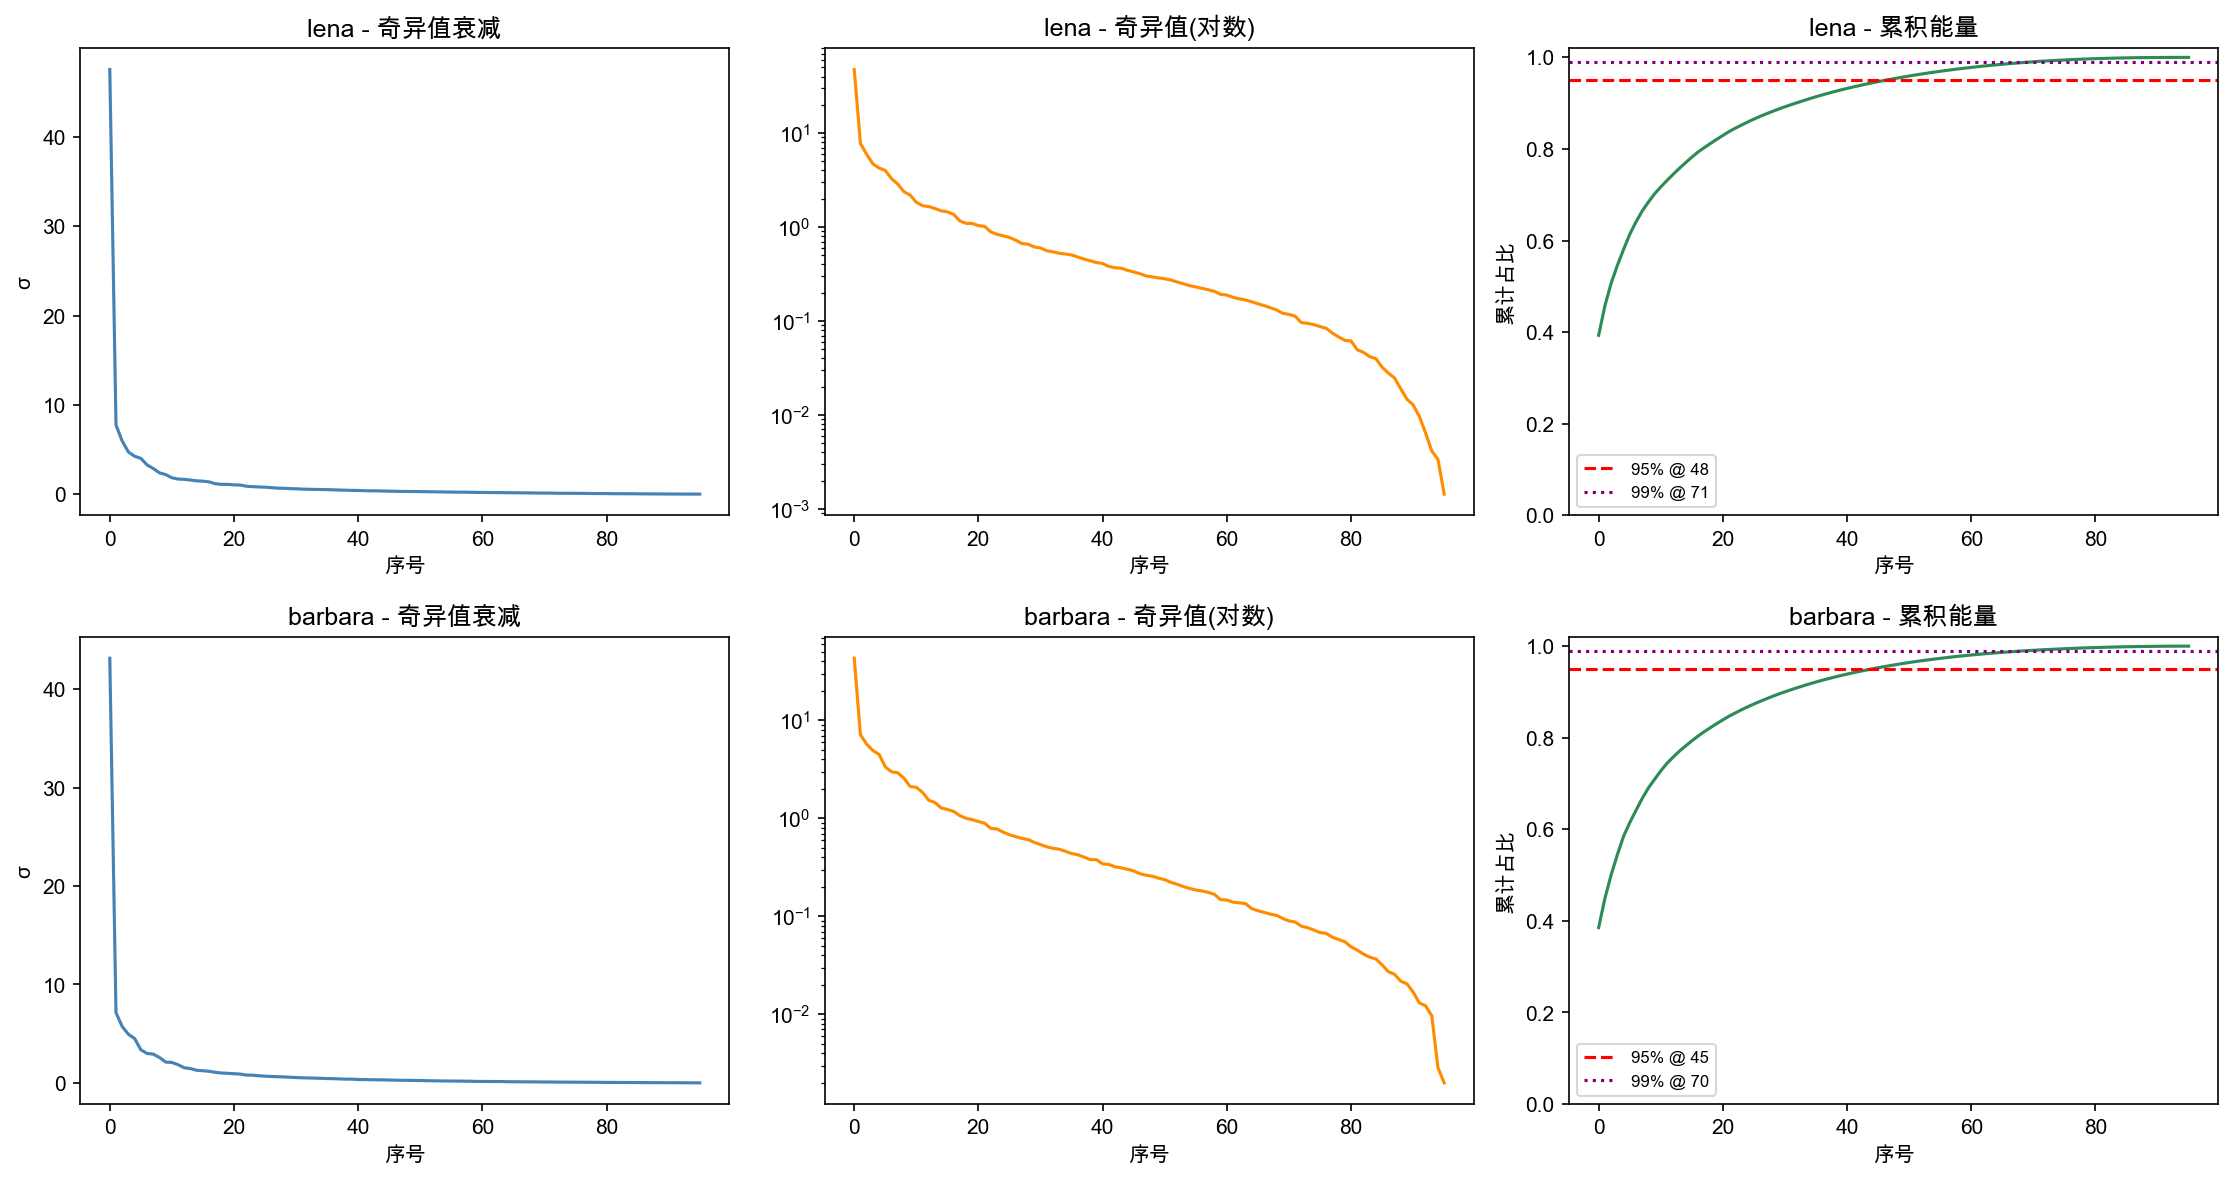
\includegraphics[width=0.85\textwidth]{figures/singular_value_overview.png}
\caption{Lena 和 Barbara 的奇异值谱与累积能量曲线。两张图的衰减模式相似，头部约 10\% 的奇异值贡献了超过 90\% 的能量，但尾部的长尾意味着完全忽略小奇异值会丢失细节。}
\label{fig:singular}
\end{figure}

图 \ref{fig:singular} 直观展示了奇异值的衰减速度。值得一提的是，Barbara 的奇异值衰减比 Lena 稍快——Barbara 图像中大面积的规则纹理（桌布、围巾）具有很强的周期性，这种结构天然适合低秩表示。而 Lena 的面部区域有较多光滑渐变，虽然也是低秩的，但中间段的奇异值衰减没那么陡。

\subsection{Patch group 的低秩性}

把低秩假设从整图缩小到局部 patch group，效果会好很多。具体做法是：选一个参考 patch，在其邻域内用块匹配找到最相似的 $K$ 个 patch，把它们展平后按行堆叠成一个 $K \times d$ 的矩阵（$d = \text{patch\_size}^2$）。由于这些 patch 本身就很相似，堆叠矩阵的秩自然很低。

\begin{figure}[H]
\centering
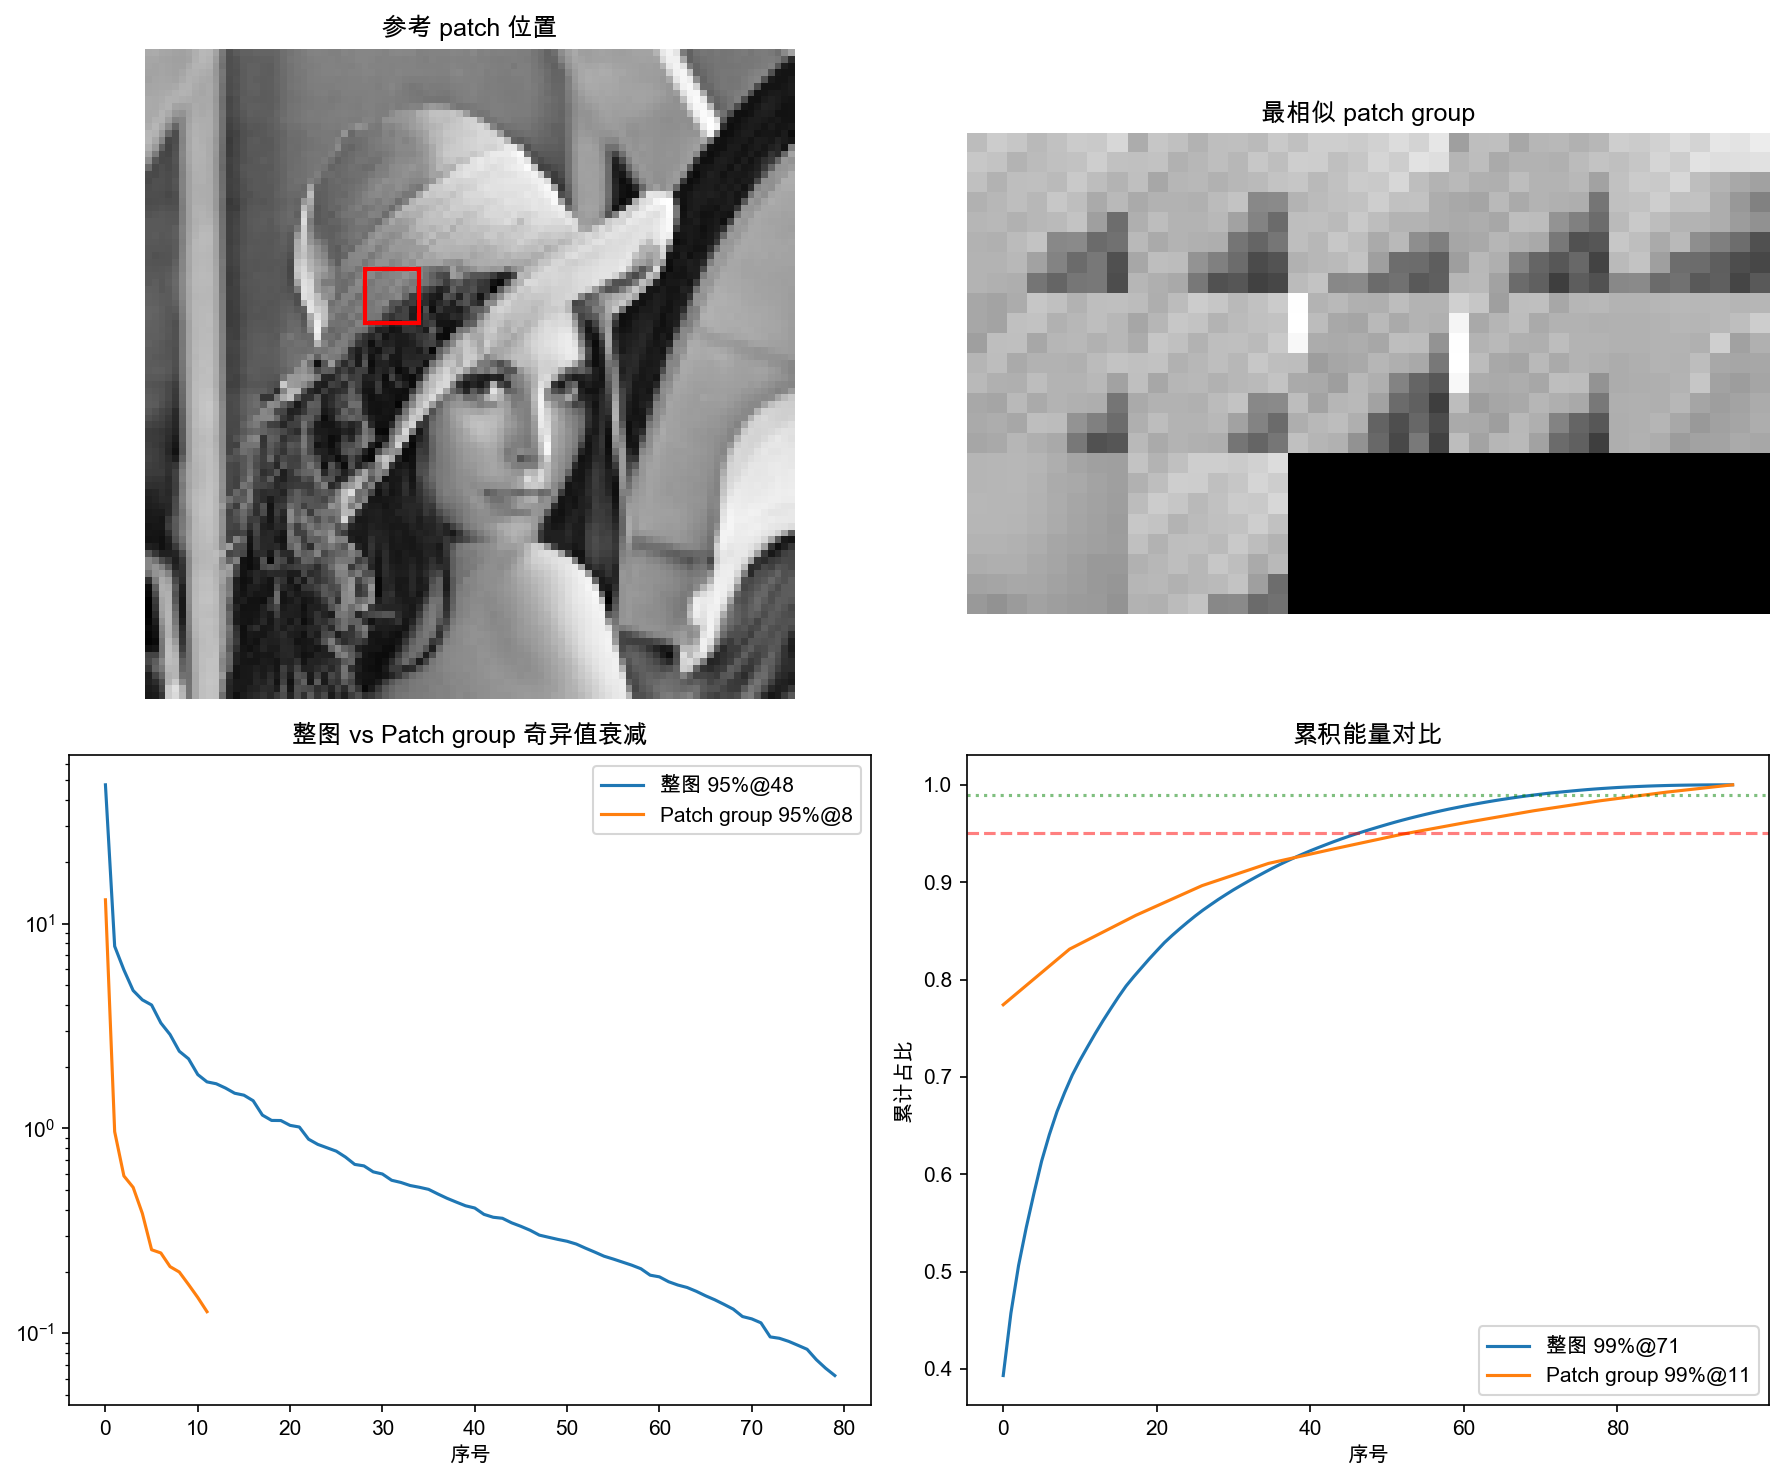
\includegraphics[width=0.9\textwidth]{figures/patch_group_rank_analysis.png}
\caption{Patch group 秩分析。左上：参考 patch 位置；右上：匹配到的相似 patch；下排：整图与 patch group 的奇异值衰减和累积能量对比。Patch group 的 95\% 能量仅需 8 个分量，远低于整图的 48 个。}
\label{fig:patch_rank}
\end{figure}

这个观察的实际意义在于：patch group 上做低秩恢复时，要估计的"自由度"少很多，同样多的观测像素能提供更充分的约束。后面 Patch-WNN 能比整图方法高 2--3\,dB，根本原因就在这里。

\subsection{退化模式与基线实验}

图 \ref{fig:patterns} 展示了本报告涉及的六种退化模式。不同模式对修复算法的挑战各不相同：随机像素缺失是最"友好"的，因为每个局部区域都有一定比例的已知像素；中心块缺失则最困难，缺失区域内完全没有观测信息。

\begin{figure}[H]
\centering
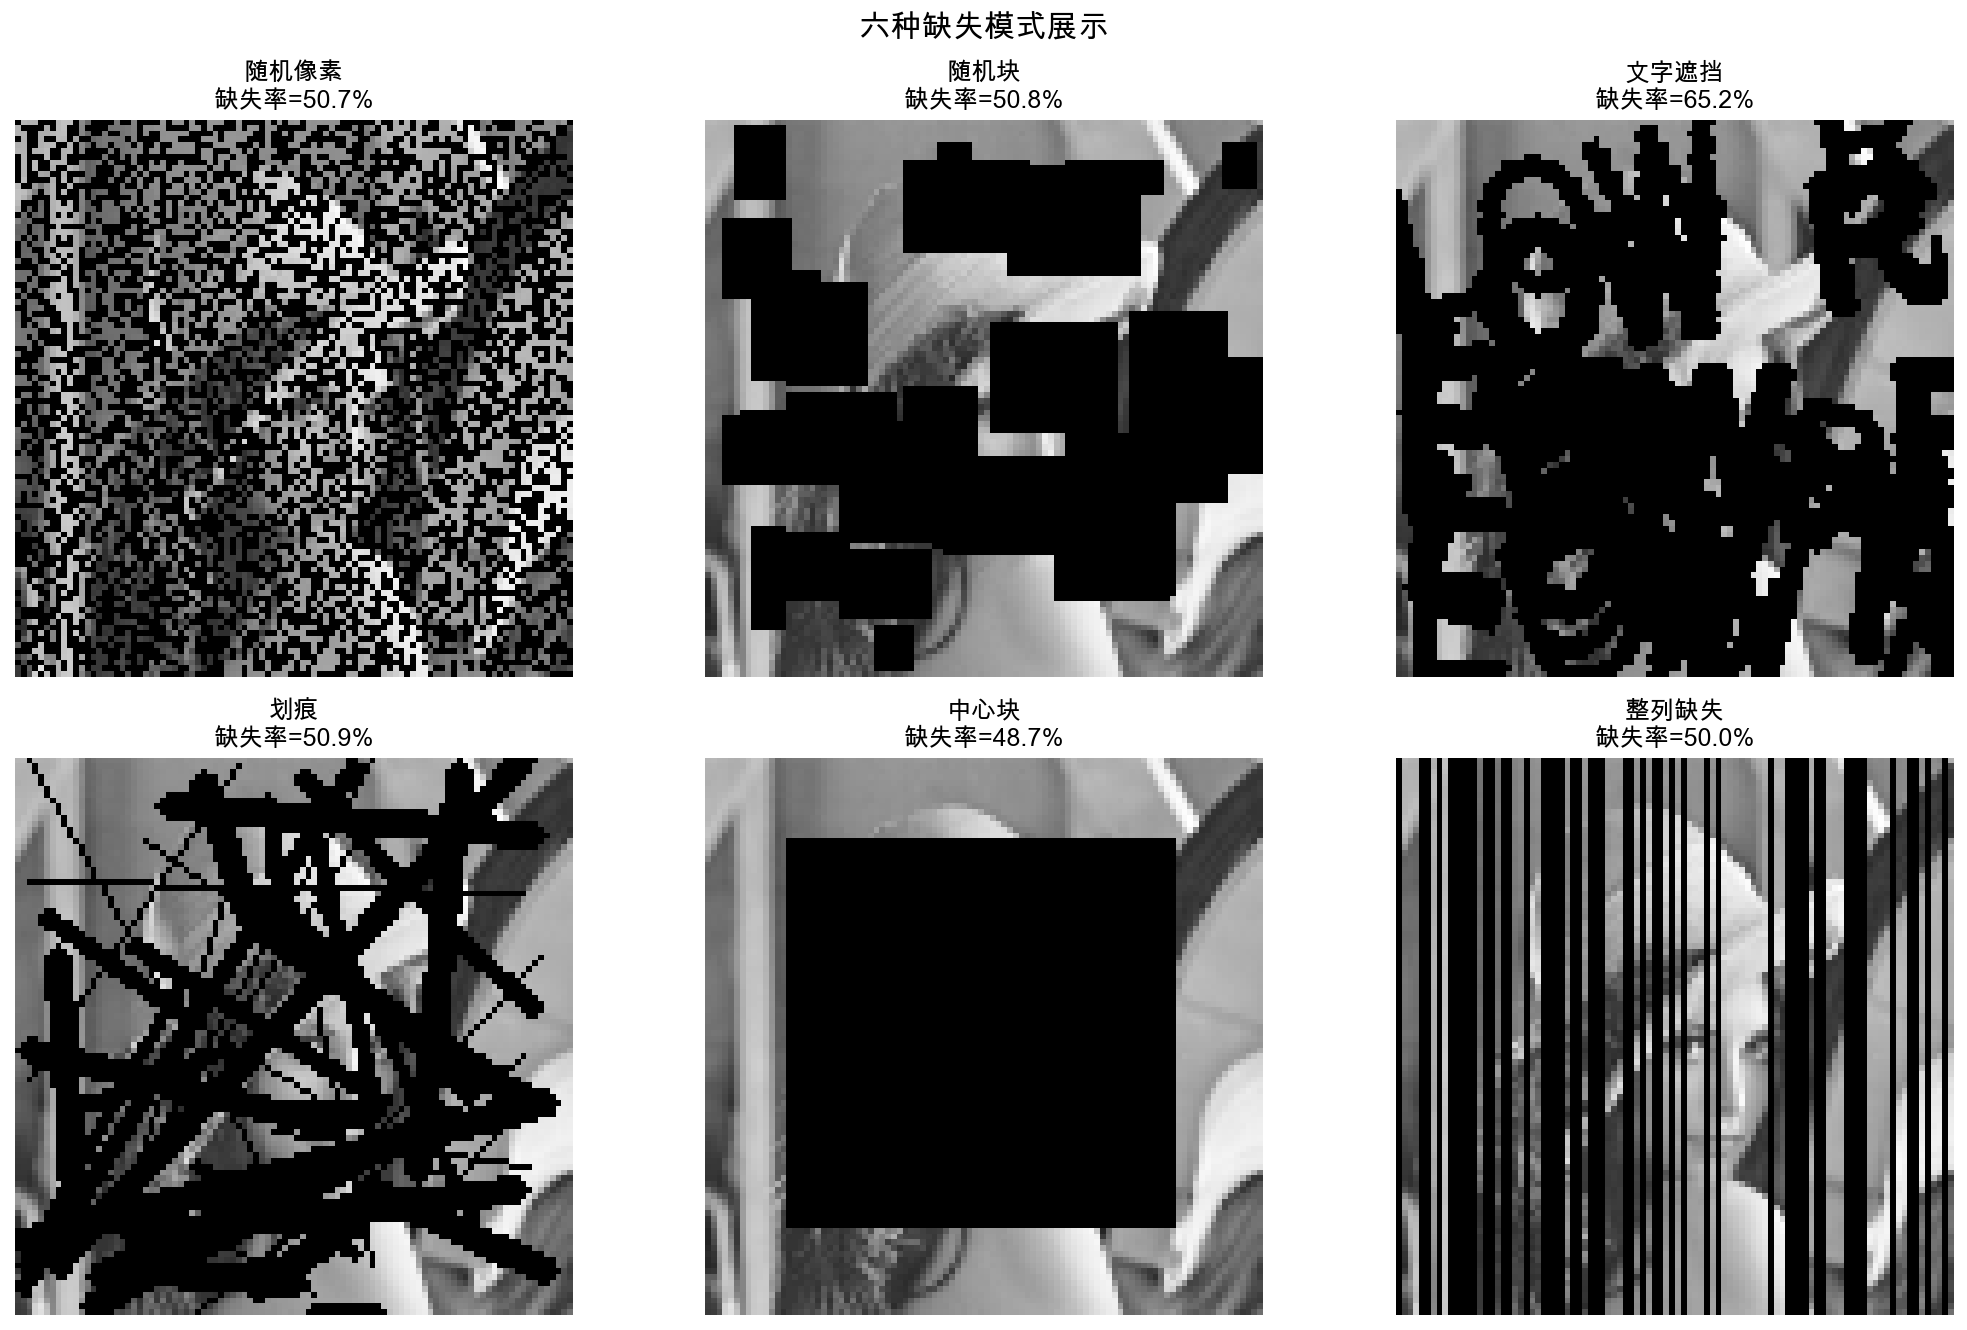
\includegraphics[width=\textwidth]{figures/missing_patterns_grid.png}
\caption{六种退化模式：随机像素、随机块、文字叠加、划痕、中心块、整列缺失。}
\label{fig:patterns}
\end{figure}

作为基线，先用最简单的截断 SVD 做修复：对观测矩阵迭代地做 rank-$k$ 近似，每次把已知位置的值固定回观测值。扫描不同的 $k$ 值，发现 $k=10$ 时 PSNR 达到峰值 23.33\,dB（图 \ref{fig:svd_baseline}）。这个数字可以理解为"整图低秩近似能做到的上限"——后续所有整图方法的 PSNR 都不会偏离这个量级太远。

\begin{figure}[H]
\centering
\begin{minipage}[t]{0.48\textwidth}
\centering
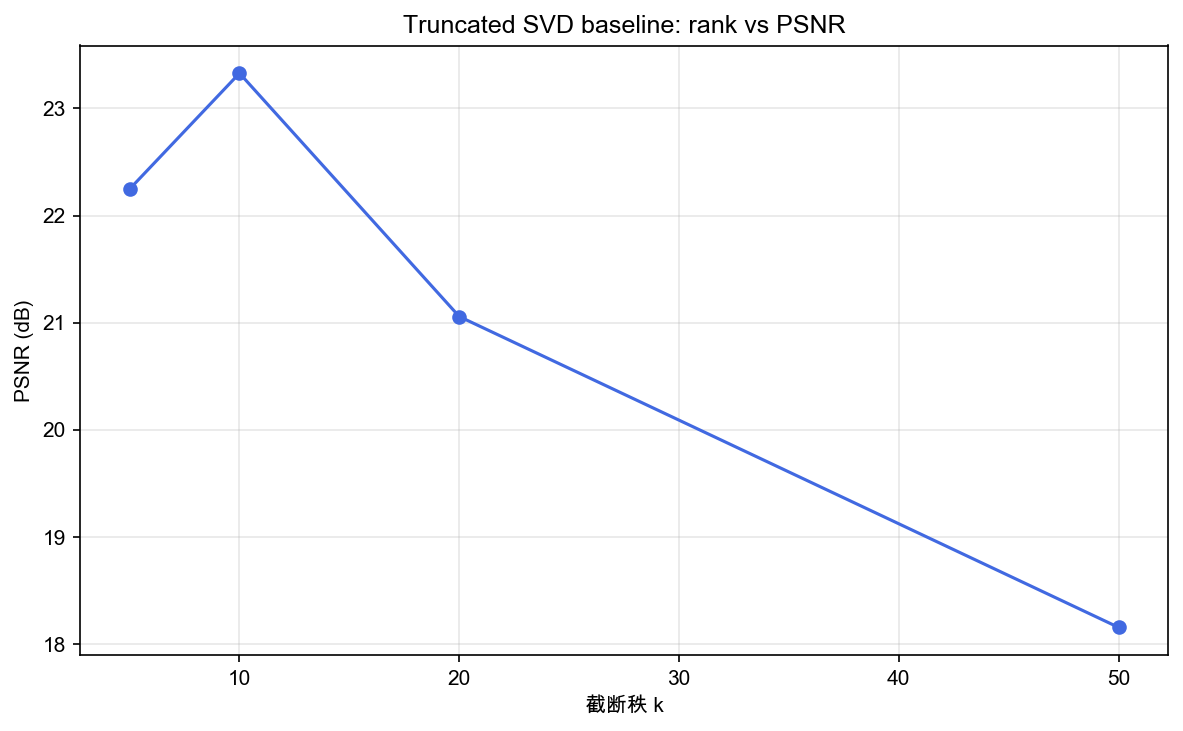
\includegraphics[width=\textwidth]{figures/truncated_svd_rank_vs_psnr.png}
\end{minipage}
\hfill
\begin{minipage}[t]{0.48\textwidth}
\centering
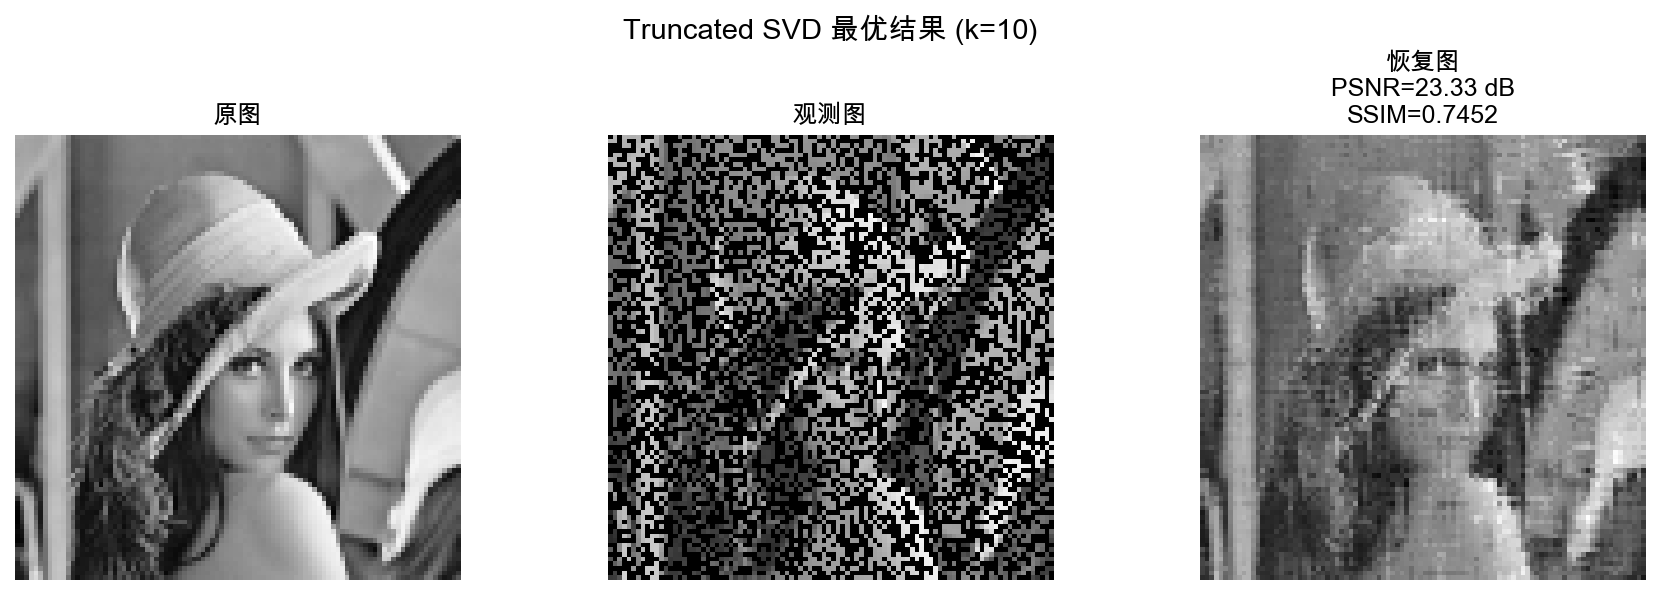
\includegraphics[width=\textwidth]{figures/truncated_svd_best.png}
\end{minipage}
\caption{截断 SVD 基线。左：不同截断秩下的 PSNR，$k=10$ 处取得最优；右：$k=10$ 的修复结果，整体结构恢复但细节偏模糊。}
\label{fig:svd_baseline}
\end{figure}

% ============================================================
\section{必做：Robust PCA}
% ============================================================

\subsection{核范数 ADMM 矩阵补全}

先从最基本的矩阵补全问题入手。直接最小化 $\operatorname{rank}(L)$ 不可行，用核范数 $\|L\|_*$ 做凸松弛后，问题变成式 (\ref{eq:nn})。这里采用 ADMM 框架求解：引入辅助变量 $Z=L$，把问题拆成两个子问题交替迭代：
\begin{equation}
    \begin{cases}
    L^{k+1} = \mathcal{D}_{1/\mu}\!\left(Z^k - Y^k/\mu\right),\\
    Z^{k+1} = \text{proj}_{P_\Omega}(L^{k+1} + Y^k/\mu, D),\\
    Y^{k+1} = Y^k + \mu(L^{k+1} - Z^{k+1}),
    \end{cases}
\end{equation}
其中 $\mathcal{D}_{\tau}(\cdot)$ 是奇异值软阈值（SVT）算子：对矩阵做 SVD，然后把每个奇异值做 $\sigma \mapsto \max(\sigma-\tau,0)$ 的收缩。$\mu$ 是增广拉格朗日的惩罚参数，每步乘以 $\rho>1$ 逐渐增大。

超参数的选择花了不少功夫。最终通过网格搜索确定 $\lambda=8.0$、初始 $\mu=0.4$、$\rho=1.05$、$\mu_{\max}=80$。这里 $\mu_{\max}$ 的设置很关键：如果不设上界，$\rho=1.1$ 跑 100 步后 $\mu$ 会膨胀到约 13780，此时 SVT 的阈值 $1/\mu$ 接近零，相当于跳过了低秩正则化，算法退化成简单的投影迭代。

\begin{figure}[H]
\centering
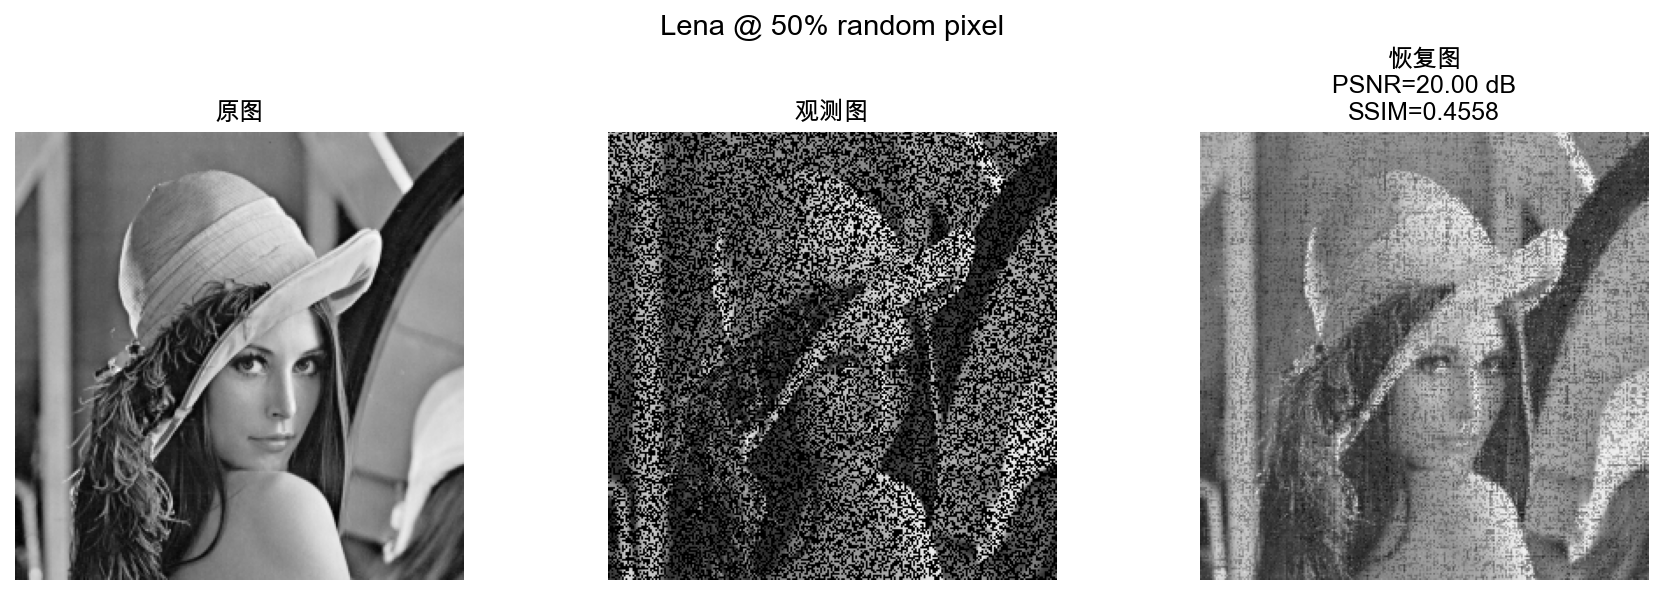
\includegraphics[width=\textwidth]{figures/lena_50_recovery.png}
\caption{Lena 50\% 随机缺失下的核范数 ADMM 修复结果。左：原图；中：观测图（黑色为缺失像素）；右：恢复图（PSNR=27.01\,dB）。}
\label{fig:lena50}
\end{figure}

\begin{figure}[H]
\centering
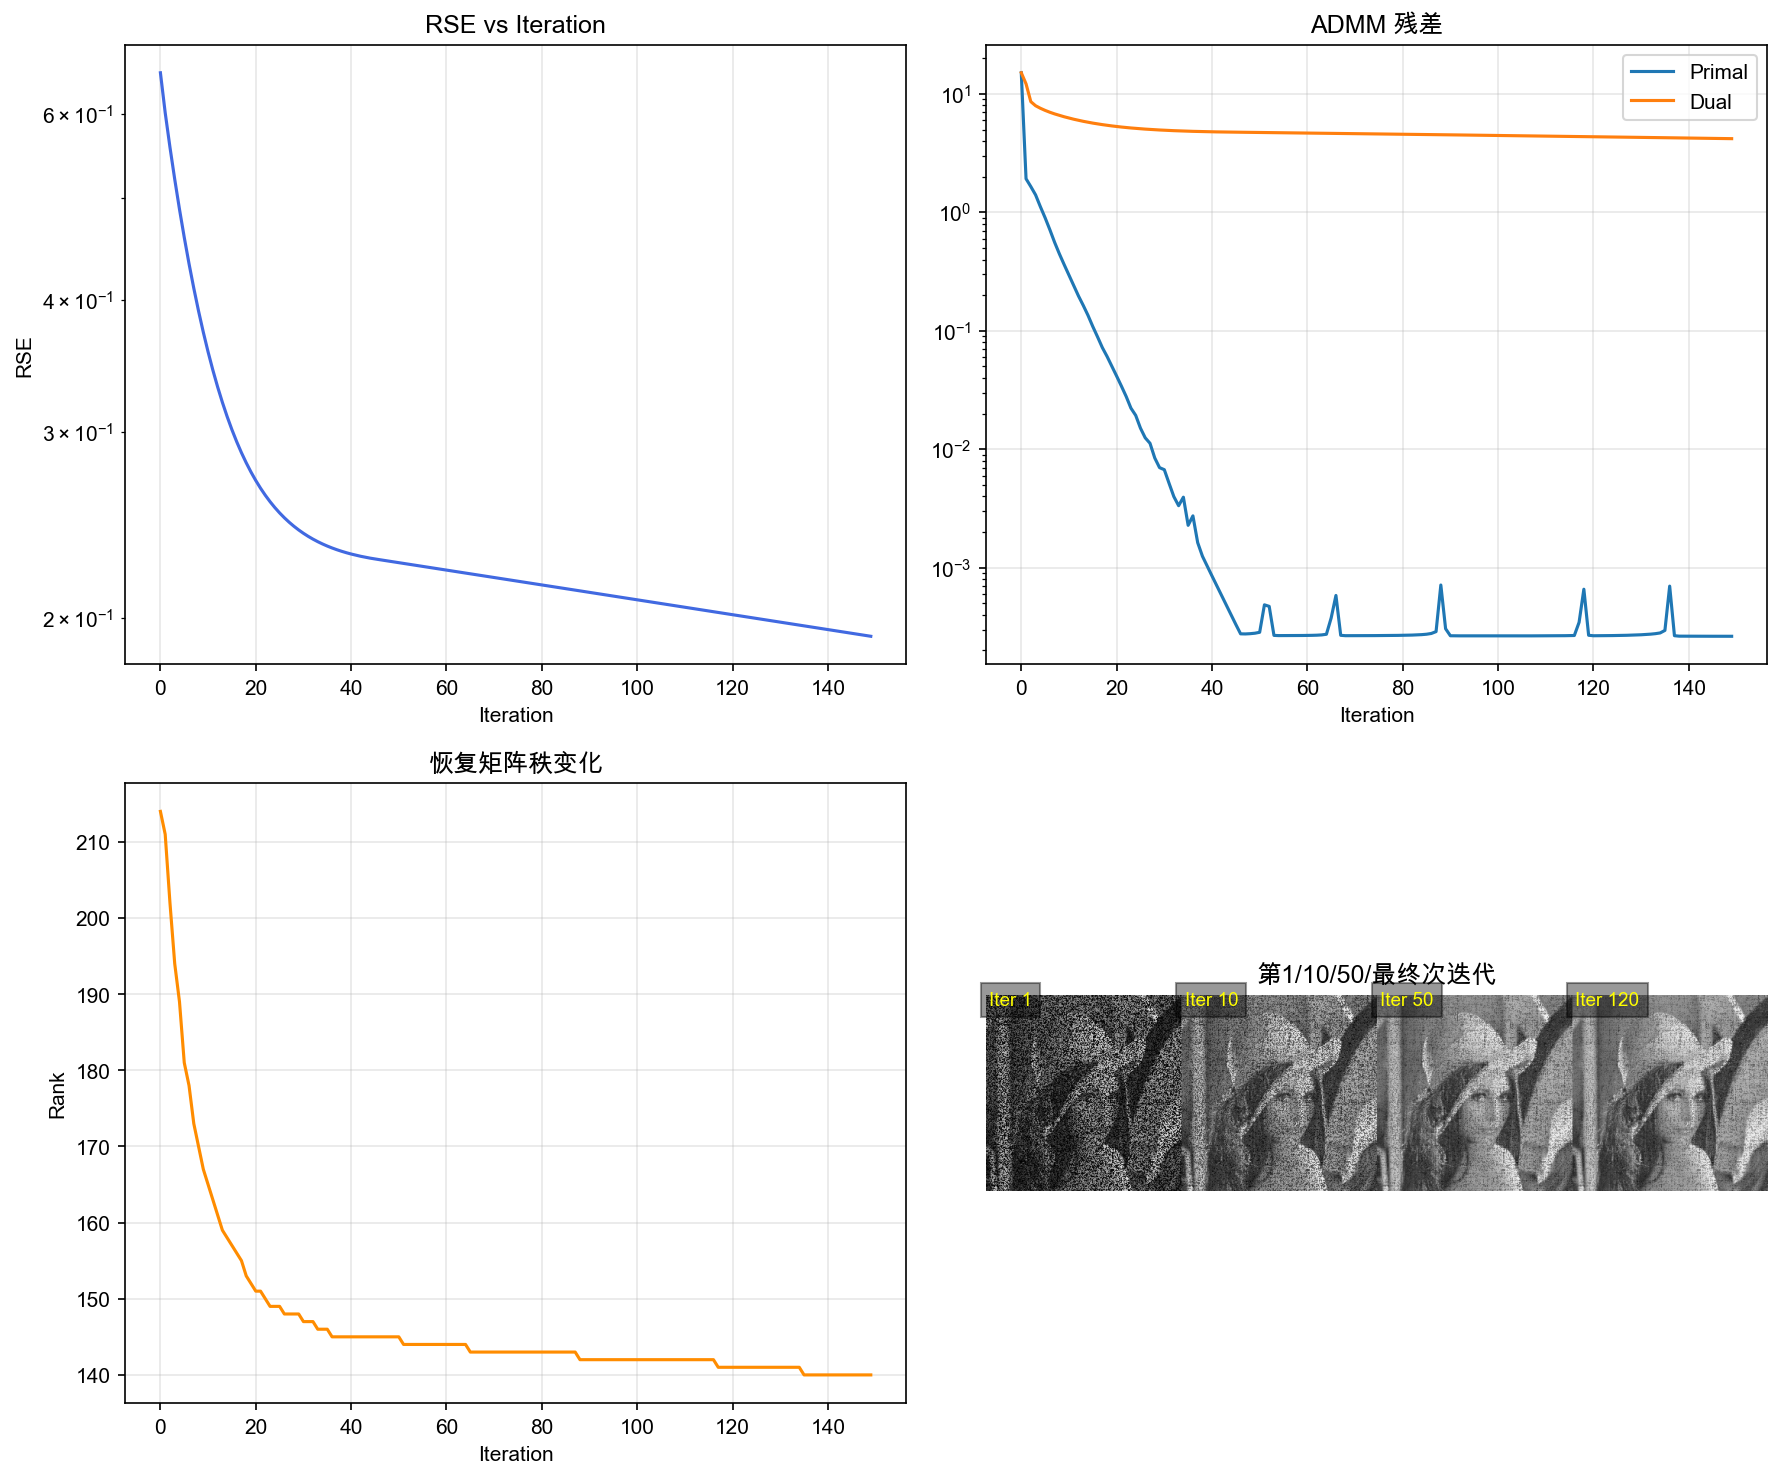
\includegraphics[width=0.85\textwidth]{figures/convergence_diagnostics.png}
\caption{ADMM 收敛诊断。左上：RSE 随迭代下降；右上：原始残差和对偶残差均按对数尺度收敛；左下：恢复矩阵的秩先升后稳定在约 60；右下：第 1/10/50/最终次迭代的恢复快照。}
\label{fig:nnadmm_conv}
\end{figure}

从收敛曲线（图 \ref{fig:nnadmm_conv}）可以看到，ADMM 大约在 60 步左右收敛。秩的变化轨迹也很有意思：初期秩快速上升（算法在"探索"合适的秩），然后稳定在 60 左右，和表 \ref{tab:effrank} 中 Lena 的 99\% 能量秩（71）大致吻合。

\subsubsection{不同缺失率下的表现}

表 \ref{tab:nnadmm_rate} 汇总了三张测试图在五个缺失率下的修复质量。

\begin{table}[H]
\centering
\caption{核范数 ADMM 在不同缺失率下的 PSNR (dB) / SSIM}
\label{tab:nnadmm_rate}
\small
\begin{tabular}{lccccc}
\toprule
图像 & 10\% & 30\% & 50\% & 70\% & 90\% \\
\midrule
Lena    & 36.97/0.974 & 31.26/0.909 & 27.01/0.793 & 22.63/0.587 & 13.67/0.158 \\
Barbara & 35.38/0.965 & 29.91/0.888 & 26.35/0.772 & 22.85/0.588 & 14.55/0.174 \\
Selfie  & 37.22/0.966 & 32.42/0.918 & 28.95/0.845 & 25.68/0.728 & 19.39/0.451 \\
\bottomrule
\end{tabular}
\end{table}

有几个现象值得讨论：

第一，质量下降的速度是非线性的。从 30\% 到 50\% 大约掉 4\,dB，但从 50\% 到 70\% 掉了 4--5\,dB，到 90\% 更是断崖式下跌。这是因为高缺失率下，每个局部区域的已知像素太少，SVT 不得不更激进地收缩奇异值，核范数对大奇异值的系统性压缩偏差就变得不可忽视了。

第二，Selfie 在所有缺失率下都表现最好，尤其是 90\% 缺失时仍有 19.39\,dB，远高于 Lena 的 13.67\,dB。这张自拍照的背景比较简单（大面积纯色），整图有效秩更低，核范数假设更贴合。

第三，Barbara 在低缺失率下和 Lena 接近，但在 70\% 以上时反而略好于 Lena。Barbara 的规则纹理虽然在视觉上看起来复杂，但从矩阵秩的角度看，周期性纹理恰恰是低秩的。

\subsubsection{参数敏感性}

图 \ref{fig:lambda} 展示了 $\lambda$ 对修复质量的影响。PSNR 在 $\lambda \in [1, 20]$ 的范围内变化不大（$\pm 1$\,dB），说明算法对这个参数不太敏感。但 $\lambda$ 过小（$<0.1$）时，观测约束太弱，恢复图偏向全零；$\lambda$ 过大（$>100$）时，核范数正则化被压制，退化成简单插值。

\begin{figure}[H]
\centering
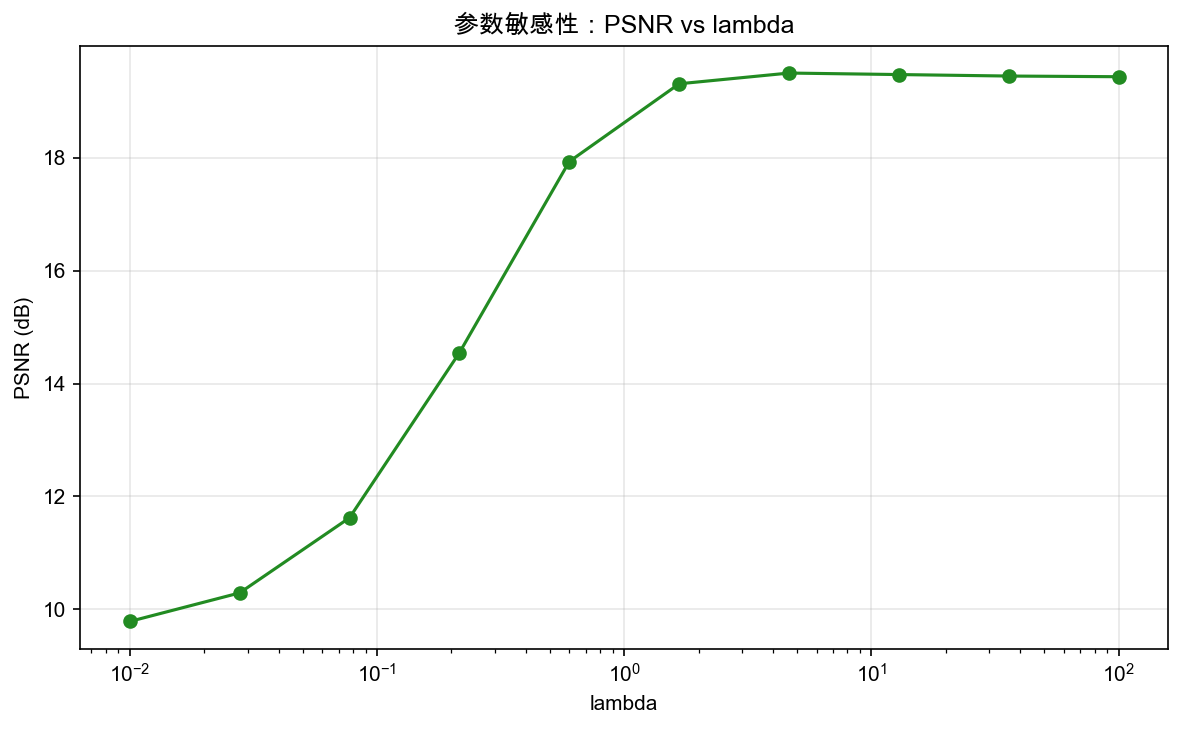
\includegraphics[width=0.65\textwidth]{figures/lambda_sensitivity.png}
\caption{$\lambda$ 参数敏感性分析。PSNR 在 $\lambda \in [1, 20]$ 范围内较为稳定。}
\label{fig:lambda}
\end{figure}

\subsection{核范数的偏差问题与非凸替代}

核范数作为秩的凸松弛虽然好优化，但有一个本质缺陷：它对所有奇异值施加相同强度的收缩。对于图像矩阵来说，前几个大奇异值承载了主要的结构信息（比如整体亮度、大尺度轮廓），它们不应该被过度压缩；而尾部的小奇异值更可能是噪声或缺失引入的伪分量，应该被强力抑制。核范数的"一视同仁"导致恢复图的奇异值谱系统性地偏小，表现为图像整体偏暗、对比度降低。

图 \ref{fig:bias} 直观展示了这个偏差：蓝色曲线是原图的奇异值，红色是核范数恢复后的奇异值，中间的红色阴影区域就是被"吃掉"的部分。

\begin{figure}[H]
\centering
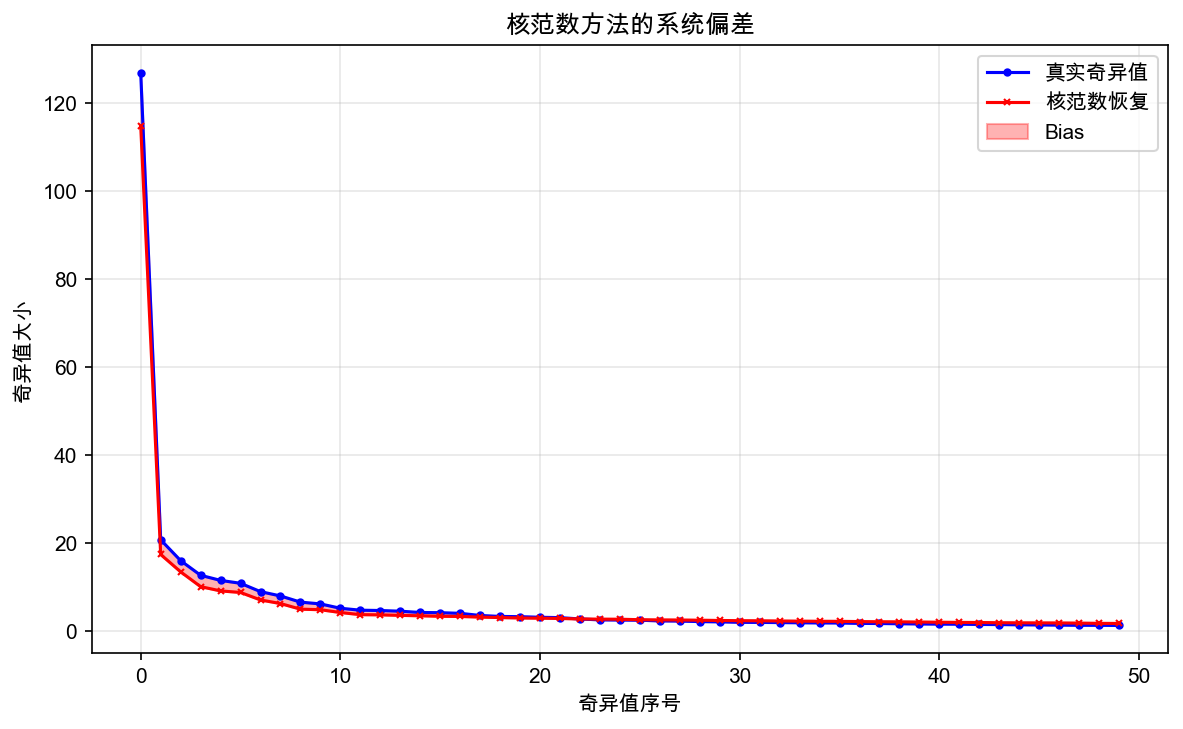
\includegraphics[width=0.75\textwidth]{figures/nuclear_norm_bias.png}
\caption{核范数的系统偏差。恢复图的奇异值在所有分量上都低于真实值，前几个主奇异值的偏差尤其明显。}
\label{fig:bias}
\end{figure}

为了缓解这个问题，可以用非凸的惩罚函数替代核范数，让大奇异值受到更小的惩罚。这里实现了两种方案：

\paragraph{Schatten-$p$ 范数} $\|L\|_{S_p}^p = \sum_i \sigma_i^p$，取 $0<p<1$。当 $p<1$ 时，$\sigma^p$ 对大 $\sigma$ 的增长速度比线性慢，相当于对大奇异值"手下留情"。对应的近端算子（广义软阈值）没有闭式解，需要用牛顿法逐分量求解。$p=0.5$ 时有一个基于三角函数的半解析公式，计算效率较好。

\paragraph{加权核范数（WNN）} $\|L\|_{w,*} = \sum_i w_i \sigma_i$，权重取 $w_i = c/(\sigma_i + \varepsilon)$。大奇异值对应小权重，几乎不被惩罚；小奇异值对应大权重，被强力收缩。这个方案的好处是近端算子仍然是逐分量的软阈值，只是阈值从统一的 $\tau$ 变成了 $w_i/\mu$，实现简单。

\begin{figure}[H]
\centering
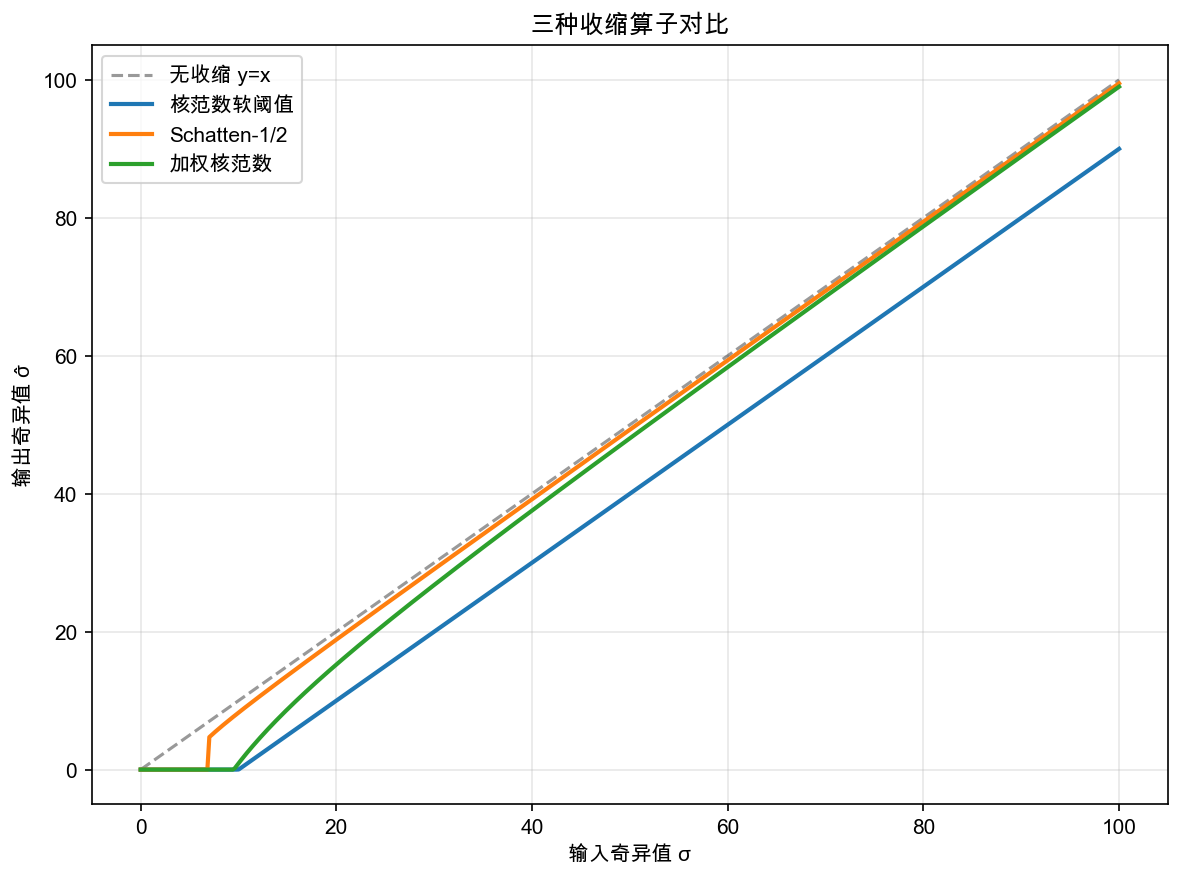
\includegraphics[width=0.75\textwidth]{figures/shrinkage_operator_comparison.png}
\caption{三种收缩算子的输入-输出关系。核范数（蓝）对所有 $\sigma$ 平移相同距离；Schatten-0.5（橙）和 WNN（绿）对大 $\sigma$ 的收缩明显减小。}
\label{fig:shrink}
\end{figure}

图 \ref{fig:p_sweep} 展示了 Schatten-$p$ 中 $p$ 值对 PSNR 的影响。$p$ 在 0.3--0.7 之间时效果优于 $p=1$（即核范数），但 $p$ 太小（如 0.1）会导致 ADMM 收敛不稳定——非凸性太强，子问题的解不唯一。

\begin{figure}[H]
\centering
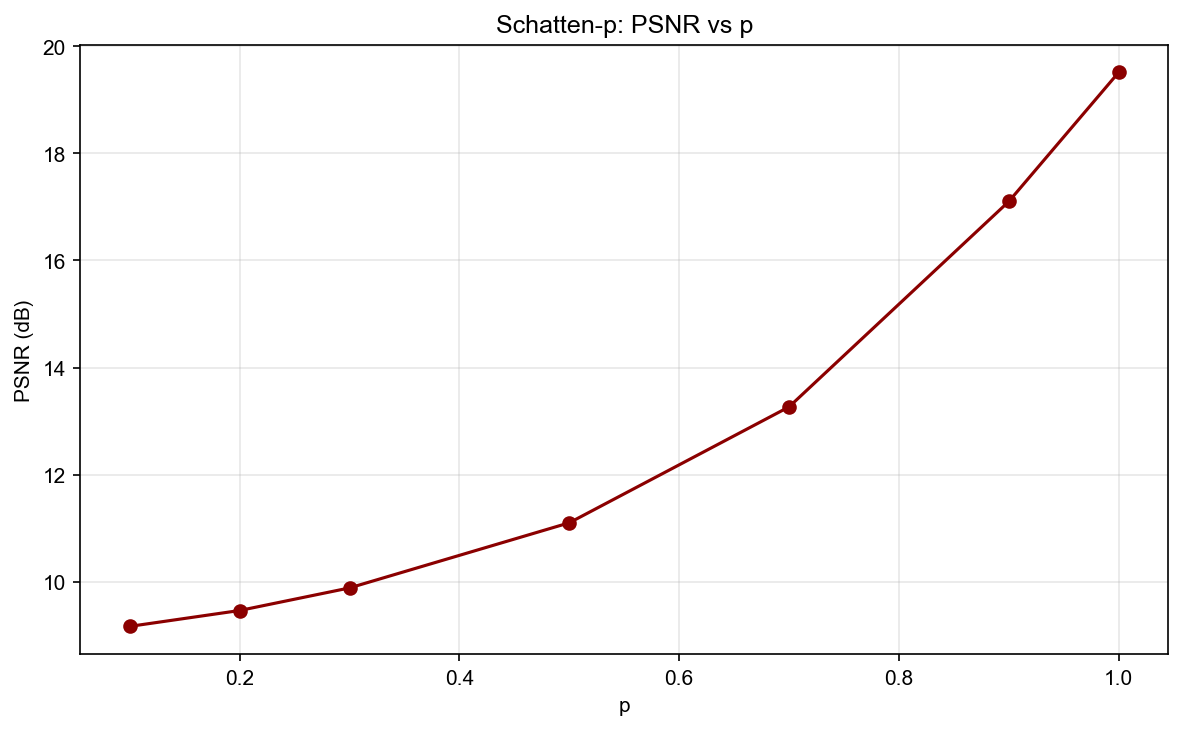
\includegraphics[width=0.65\textwidth]{figures/p_vs_psnr.png}
\caption{Schatten-$p$ 的 $p$ 值扫描。$p \in [0.3, 0.7]$ 是比较好的区间。}
\label{fig:p_sweep}
\end{figure}

\begin{table}[H]
\centering
\caption{三种收缩方案在 50\% 随机缺失下的 PSNR/SSIM}
\label{tab:shrink}
\begin{tabular}{lccc}
\toprule
图像 & 核范数 & Schatten-0.5 & WNN \\
\midrule
Lena    & \textbf{27.07}/0.794 & 26.26/0.716 & 25.95/0.703 \\
Barbara & \textbf{26.41}/0.769 & 25.36/0.702 & 24.76/0.678 \\
Selfie  & \textbf{29.24}/0.844 & 28.31/0.747 & 27.79/0.746 \\
\bottomrule
\end{tabular}
\end{table}

表 \ref{tab:shrink} 的结果可能有点出乎意料：在整图层面上，非凸替代反而不如核范数。这并不是说 WNN 或 Schatten-$p$ 本身有问题，而是整图的有效秩在 40--50 之间，非凸替代能"修正"的偏差空间很有限，稍微调过头就会破坏恢复质量。后面把同样的 WNN 算子搬到 Patch group 上时（有效秩只有 8--11），情况会完全不同。

\begin{figure}[H]
\centering
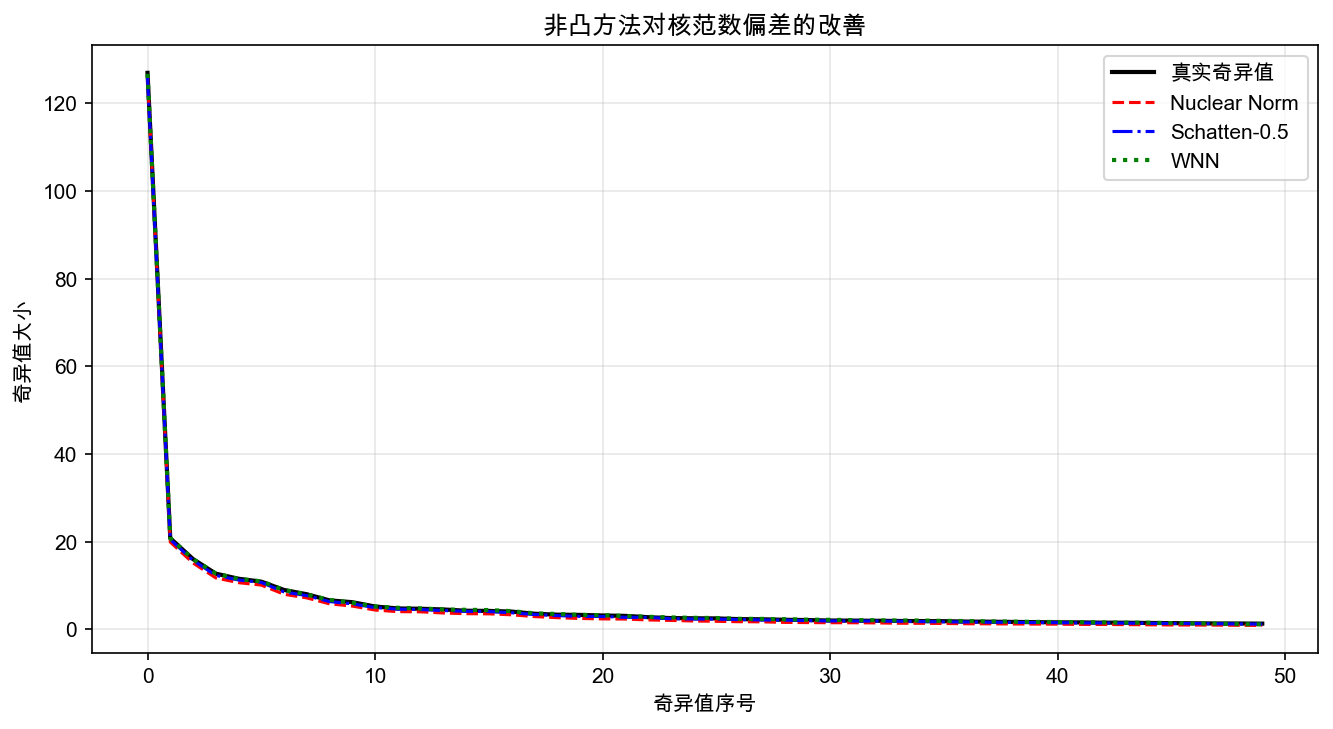
\includegraphics[width=0.75\textwidth]{figures/bias_improvement.png}
\caption{三种方法恢复后的奇异值谱对比。WNN 在前几个主奇异值上确实更接近真实值，但整图尺度上这个优势还不够大。}
\label{fig:bias_improve}
\end{figure}

\subsection{RPCA：低秩 + 稀疏分解}

前面的核范数 ADMM 处理的是"缺失"——像素值未知，用掩码标记。但实际场景中还有一类退化是"污染"——像素值被替换成了别的东西（比如文字覆盖、划痕），原始值丢失了但位置上有一个错误的观测。这时候纯核范数模型就不够用了，因为它假设观测位置的值是准确的。

Robust PCA \cite{candes2011rpca} 正是为这种情况设计的。它把观测矩阵 $D$ 分解为低秩部分 $L$（主体结构）和稀疏部分 $S$（污染）：
\begin{equation}
    \min_{L,S}\; \|L\|_* + \lambda \|S\|_1 \quad \text{s.t.}\quad D = L + S,
    \quad \lambda = 1/\sqrt{\max(m,n)}.
\end{equation}
$\lambda$ 的默认取值 $1/\sqrt{\max(m,n)}$ 来自理论分析，在实践中通常不需要调。求解采用 inexact ALM（iALM）\cite{lin2010alm}：

\begin{algorithm}[H]
\caption{RPCA via iALM}
\begin{algorithmic}[1]
\REQUIRE 观测 $D$，参数 $\lambda$，初值 $\mu = 1.25/\|D\|_2$
\STATE 初始化 $S = 0, Y = 0$
\FOR{$k = 1, 2, \ldots$}
    \STATE $L \leftarrow \mathcal{D}_{1/\mu}\!\big(D - S + Y/\mu\big)$ \COMMENT{SVT：收缩奇异值}
    \STATE $S \leftarrow \mathcal{S}_{\lambda/\mu}\!\big(D - L + Y/\mu\big)$ \COMMENT{软阈值：收缩矩阵元素}
    \STATE $Y \leftarrow Y + \mu (D - L - S)$
    \STATE $\mu \leftarrow \min(\rho\mu, \mu_{\max})$
    \STATE 若 $\|D-L-S\|_F/\|D\|_F < \text{tol}$ 则终止
\ENDFOR
\end{algorithmic}
\end{algorithm}

和核范数 ADMM 的区别在于多了一个 $S$ 的更新步，用的是逐元素的软阈值 $\mathcal{S}_\tau(x) = \text{sign}(x)\max(|x|-\tau, 0)$。直觉上，$L$ 步把"大部分像素都差不多"的成分提取出来，$S$ 步把"少数像素偏离很大"的成分剥离出去。

\begin{figure}[H]
\centering
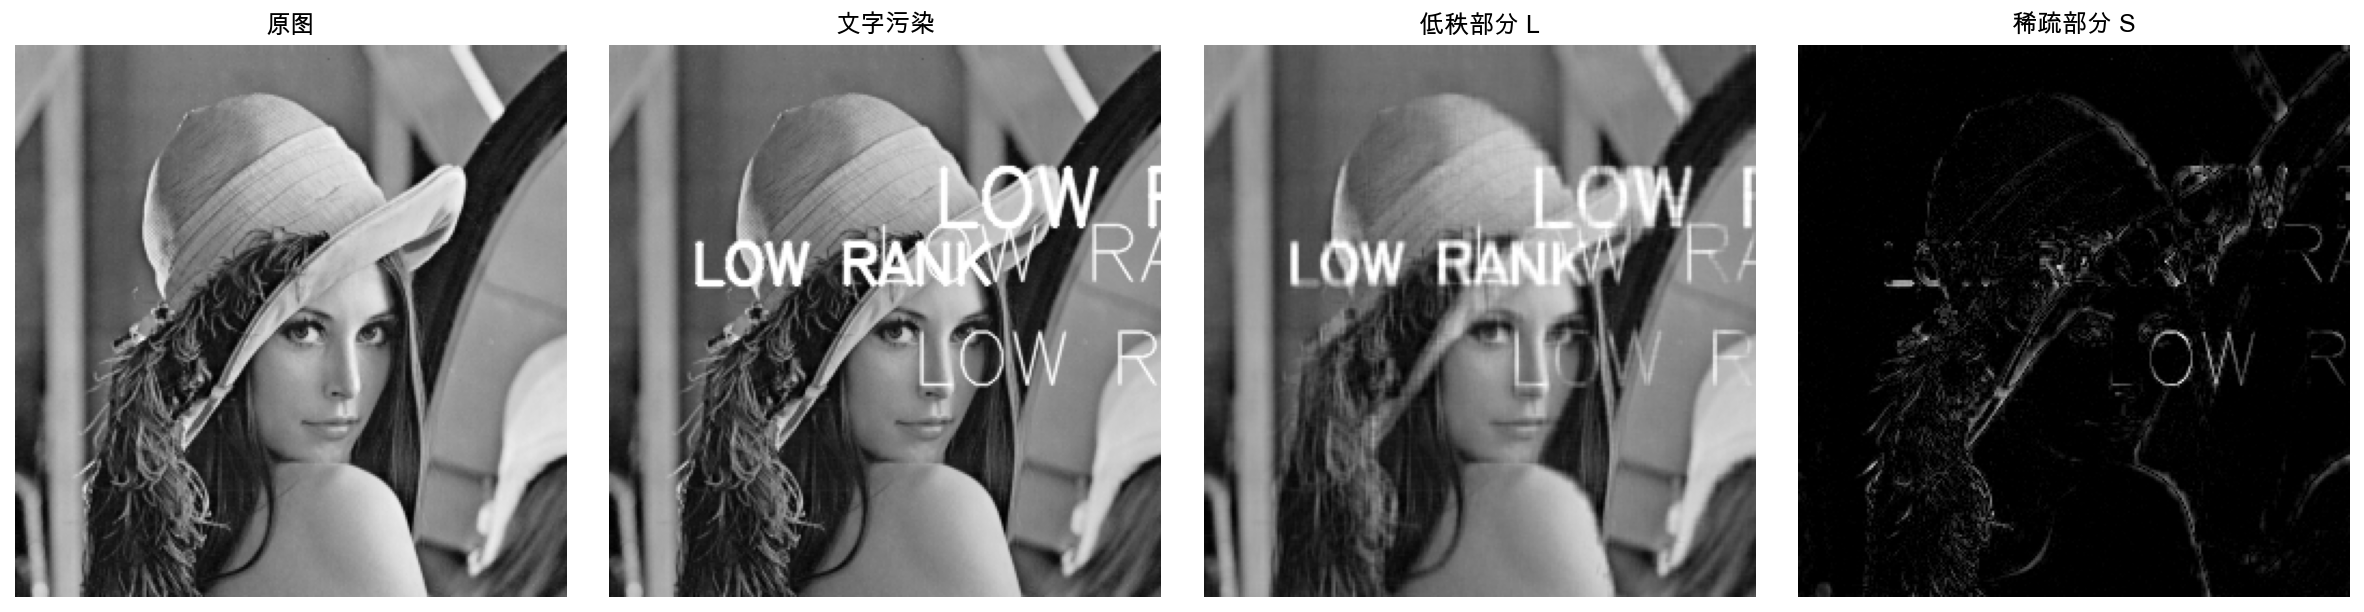
\includegraphics[width=\textwidth]{figures/rpca_text_removal.png}
\caption{RPCA 文字分离效果。从左到右：原图、文字污染图、低秩部分 $L$、稀疏部分 $|S|$。$S$ 几乎只保留了文字笔画的轮廓，$L$ 恢复了干净的背景。}
\label{fig:rpca_text}
\end{figure}

图 \ref{fig:rpca_text} 的效果相当直观：RPCA 成功地把文字"剥"了出来。不过仔细看 $L$ 会发现，文字覆盖区域的恢复并不完美——有轻微的模糊和色差，这是因为 RPCA 只做了一次全局分解，没有利用局部纹理的自相似性。

RPCA 的另一个经典应用是视频前景/背景分离。把视频的每一帧展平成一列，堆成矩阵后做 $L+S$ 分解：$L$ 对应静态背景（各帧几乎相同，所以低秩），$S$ 对应运动前景（只在少数像素位置出现，所以稀疏）。

\begin{figure}[H]
\centering
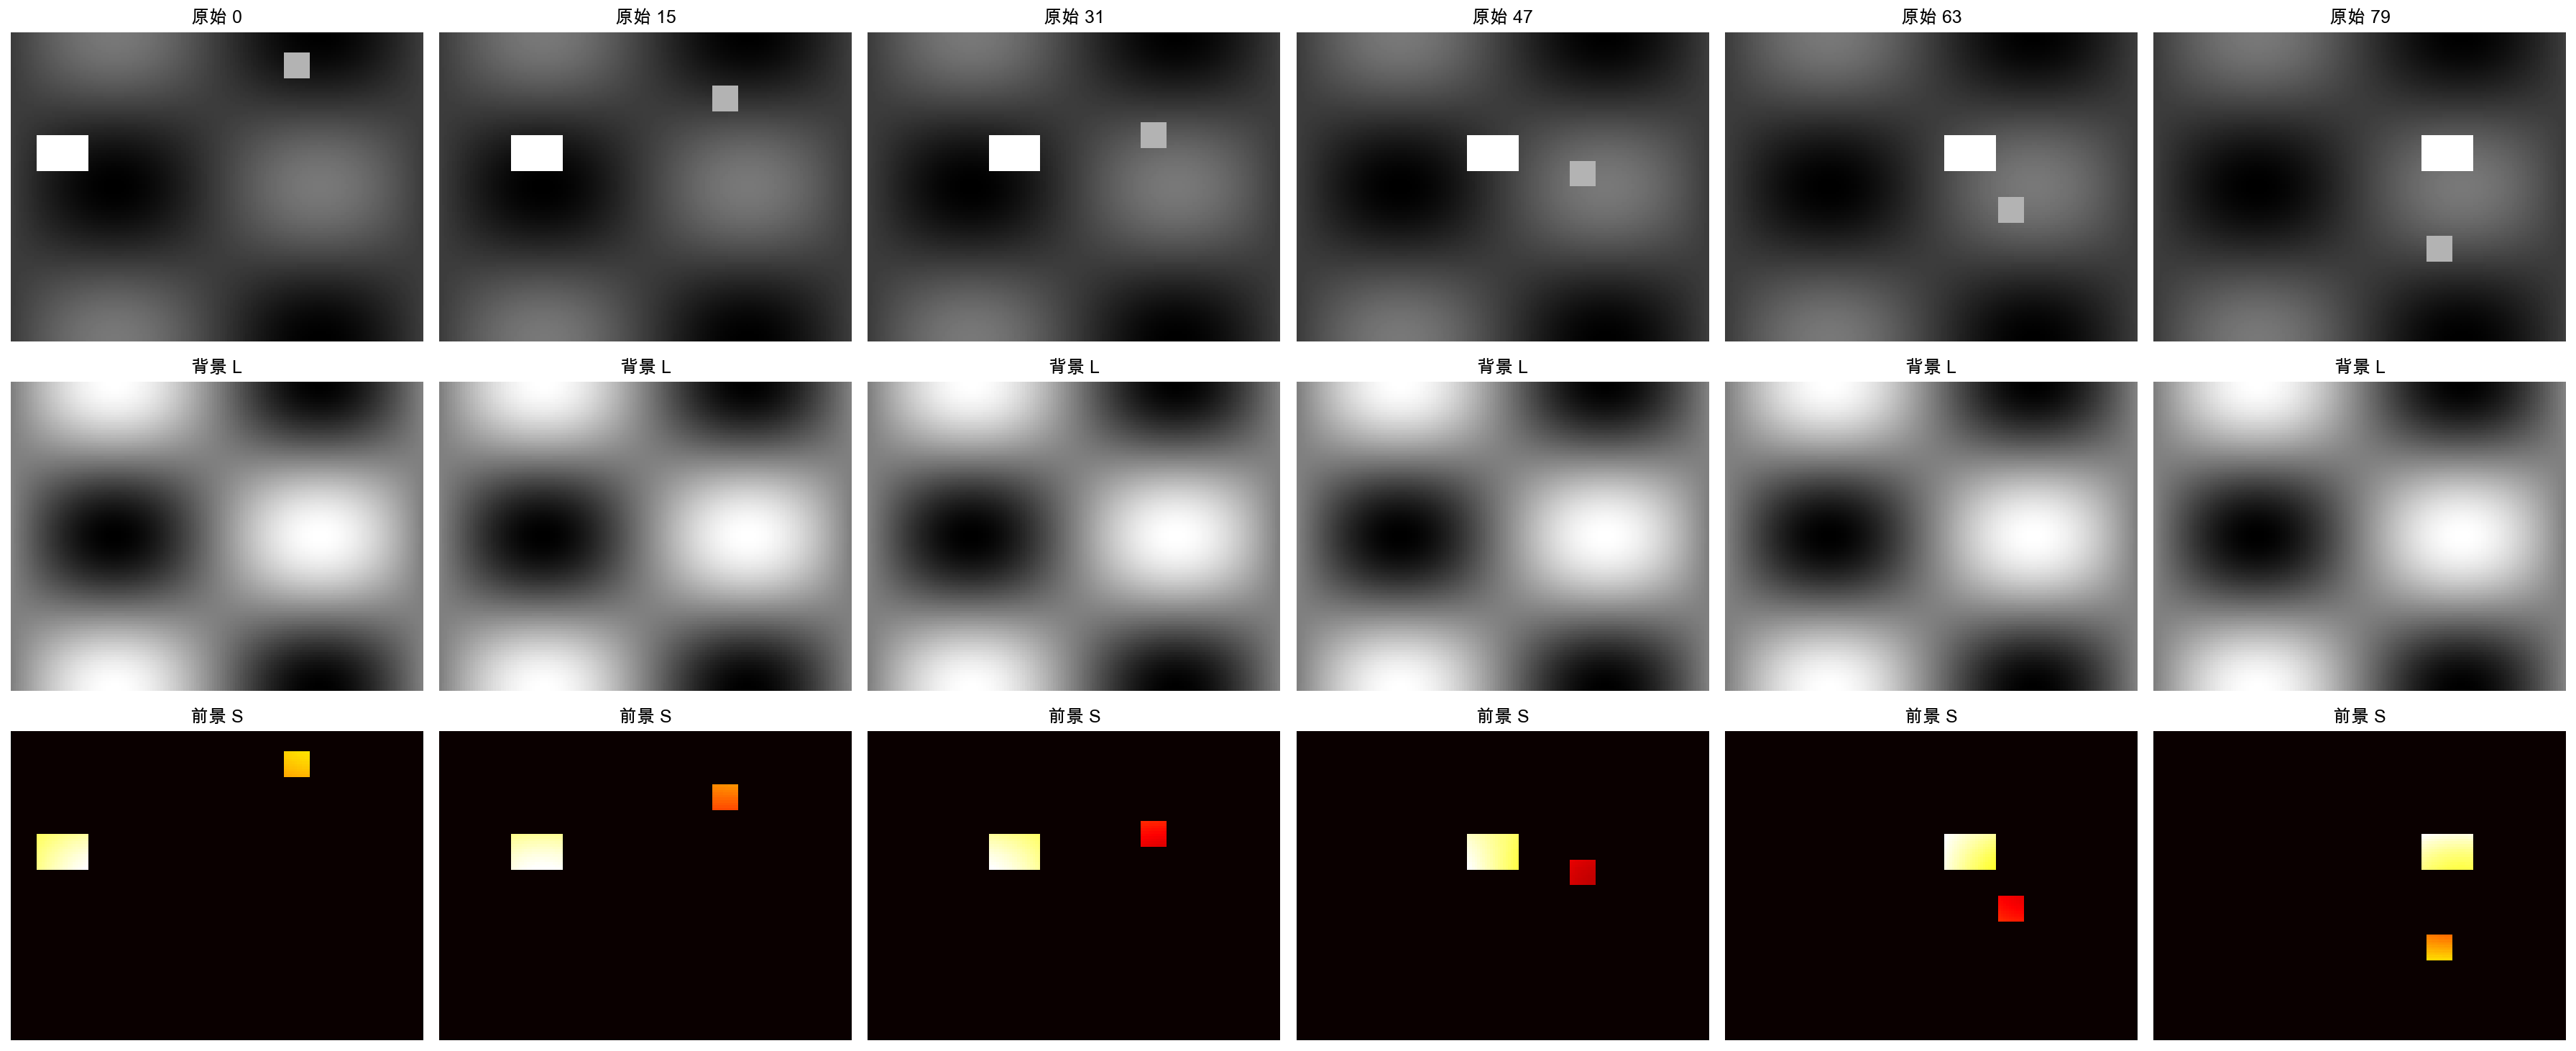
\includegraphics[width=0.85\textwidth]{figures/video_background_separation.png}
\caption{RPCA 视频背景分离。上排：原始帧；中排：低秩部分（背景）；下排：稀疏部分（前景运动目标）。}
\label{fig:video}
\end{figure}

\subsection{RPCA 的适用边界}
\label{sec:rpca_boundary}

RPCA 的核心假设是污染部分 $S$ 是稀疏的。那么当这个假设不成立时会怎样？为此测试了四种不同的退化模式：

\begin{table}[H]
\centering
\caption{RPCA 在不同退化模式下的修复质量（Lena）}
\label{tab:rpca_apply}
\begin{tabular}{lccl}
\toprule
退化模式 & PSNR (dB) & SSIM & 稀疏性分析 \\
\midrule
划痕       & 22.26 & 0.833 & 线条细且稀疏，最符合假设 \\
文字叠加   & 20.09 & 0.805 & 笔画较密，边缘处稀疏性受损 \\
随机像素   & 18.09 & 0.432 & 逐像素稀疏但无结构，$S$ 难以定位 \\
中心块缺失 & 18.47 & 0.719 & 完全不稀疏，RPCA 无法处理 \\
\bottomrule
\end{tabular}
\end{table}

\begin{figure}[H]
\centering
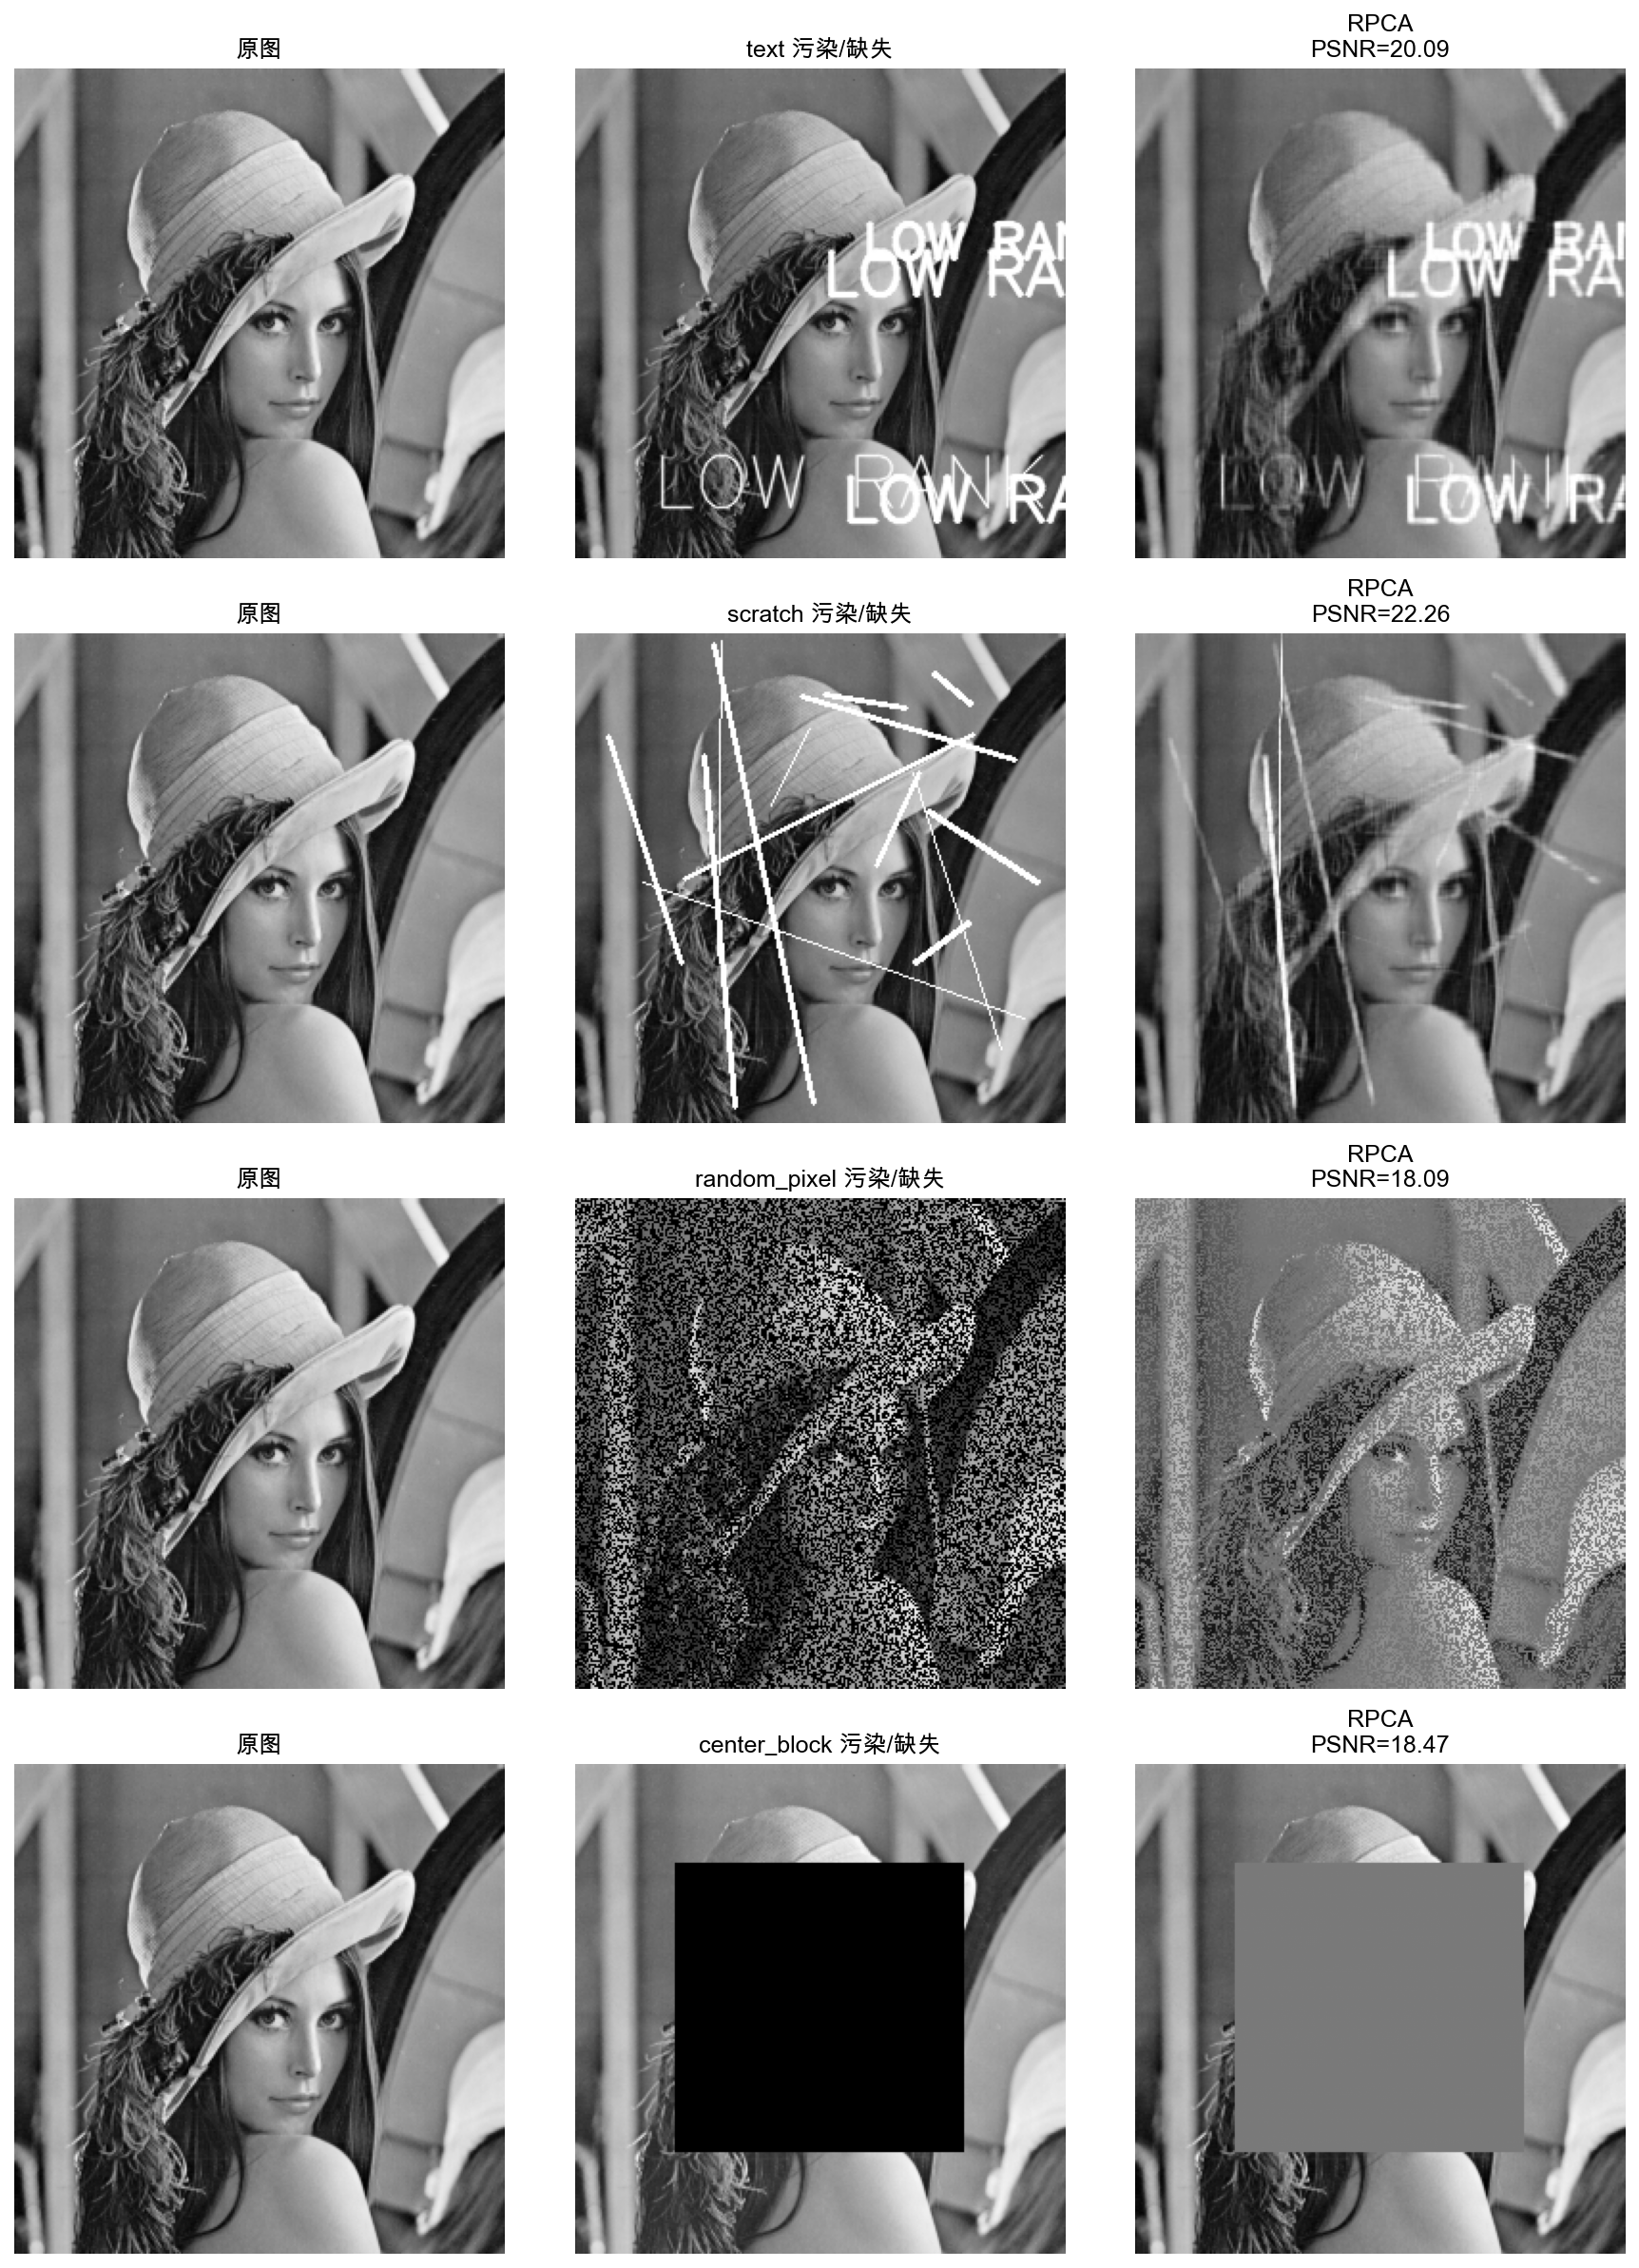
\includegraphics[width=\textwidth]{figures/rpca_applicability.png}
\caption{RPCA 在四种退化模式下的恢复对比。划痕场景效果最好；中心块缺失时 $S$ 无法表达整块缺失，$L$ 只能靠全局低秩近似来"猜"。}
\label{fig:rpca_apply}
\end{figure}

结果很清楚：划痕是 RPCA 最擅长的场景，因为划痕同时满足"稀疏"和"幅值大"两个条件，$S$ 能精准地把它们挑出来。文字叠加稍差一些，因为文字笔画比较密集，局部区域的"稀疏性"被破坏了。随机像素缺失虽然从全局看是稀疏的，但 RPCA 不知道哪些像素是缺失的（没有掩码信息），只能盲目地做 $L+S$ 分解，效果自然有限。中心块缺失则完全违反稀疏假设——一整块区域都是缺失的，$S$ 根本无法表达。

这里有一个实践中很重要的教训：\textbf{如果已知污染位置的掩码，就应该把它用上}，而不是让 RPCA 自己去猜。在后面的 GUI 实现中，把 RPCA 嵌入迭代框架——每次 $L+S$ 分解后将已知干净位置投影回观测值——文字和划痕的 PSNR 从 14--18\,dB 提升到了 24--26\,dB。

\subsection{从整图到 Patch：局部低秩先验}
\label{sec:patch}

前面的所有方法都是在整图矩阵上操作的，受限于整图有效秩较高（$\sim$45--70），修复质量有天花板。一个自然的改进思路是：把低秩假设从整图缩小到局部 patch group。

具体做法是：对图像中每个位置，提取一个 $8\times 8$ 的参考 patch，在其邻域内用块匹配（block matching）找到最相似的 $K$ 个 patch，把它们展平后堆叠成 $K \times 64$ 的矩阵，然后在这个小矩阵上做低秩恢复（SVT 或 WNN 收缩），最后把恢复后的 patch 写回原图。所有位置处理完后做加权平均，算一轮；重复若干轮直到收敛。

\begin{table}[H]
\centering
\caption{整图方法与 Patch 方法对比（50\% 随机缺失）}
\label{tab:whole_patch}
\small
\begin{tabular}{lcccccc}
\toprule
方法 & \multicolumn{2}{c}{Lena} & \multicolumn{2}{c}{Barbara} & \multicolumn{2}{c}{Selfie} \\
\cmidrule(lr){2-3} \cmidrule(lr){4-5} \cmidrule(lr){6-7}
     & PSNR & SSIM & PSNR & SSIM & PSNR & SSIM \\
\midrule
Whole-NNM  & 26.83 & 0.792 & 26.26 & 0.767 & 29.26 & 0.845 \\
Whole-WNN  & 25.96 & 0.707 & 24.63 & 0.673 & 27.85 & 0.748 \\
Patch-soft & 20.56 & 0.620 & 20.90 & 0.609 & 23.08 & 0.805 \\
Patch-WNN  & \textbf{29.37} & \textbf{0.912} & \textbf{28.63} & \textbf{0.882} & \textbf{29.11} & \textbf{0.899} \\
\bottomrule
\end{tabular}
\end{table}

表 \ref{tab:whole_patch} 的结果很有意思。首先，Patch-WNN 在所有图像上都是最好的，Lena 上达到 29.37\,dB，比整图核范数高出 2.5\,dB。其次，Patch-soft（用核范数软阈值做 patch 级收缩）反而比整图方法差——这再次印证了前面的分析：核范数的均匀收缩在低秩环境下偏差更大，patch group 的有效秩只有 8--11，核范数把前几个关键分量压得太狠了。换成 WNN 后，大奇异值被保护，效果立刻上来。

\begin{figure}[H]
\centering
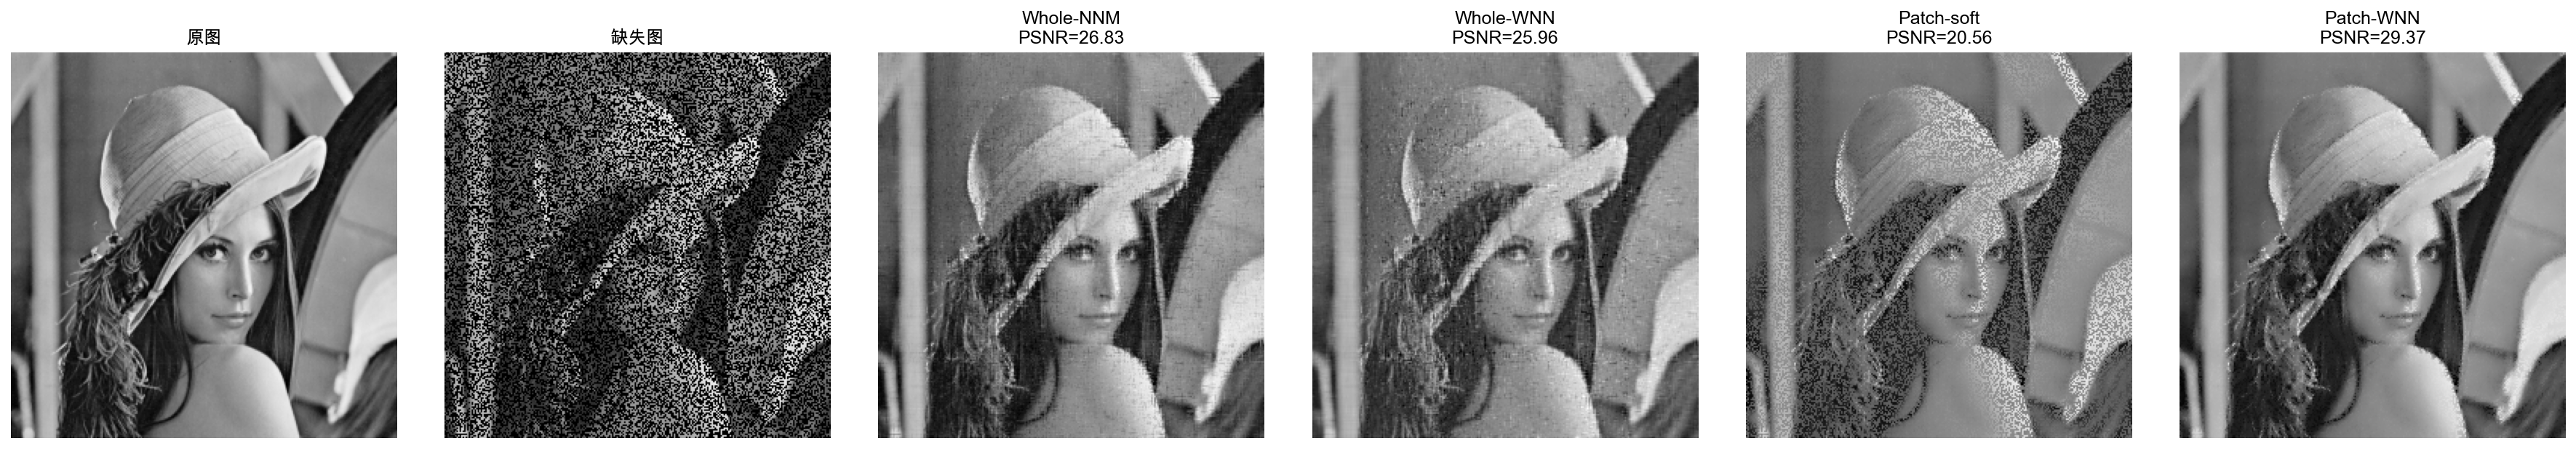
\includegraphics[width=\textwidth]{figures/whole_vs_patch_lena.png}
\caption{Lena 50\% 缺失下各方法对比。整图方法保留了全局结构但细节偏软；Patch-WNN 利用局部自相似先验恢复了更多纹理细节。}
\label{fig:whole_vs_patch}
\end{figure}

\begin{figure}[H]
\centering
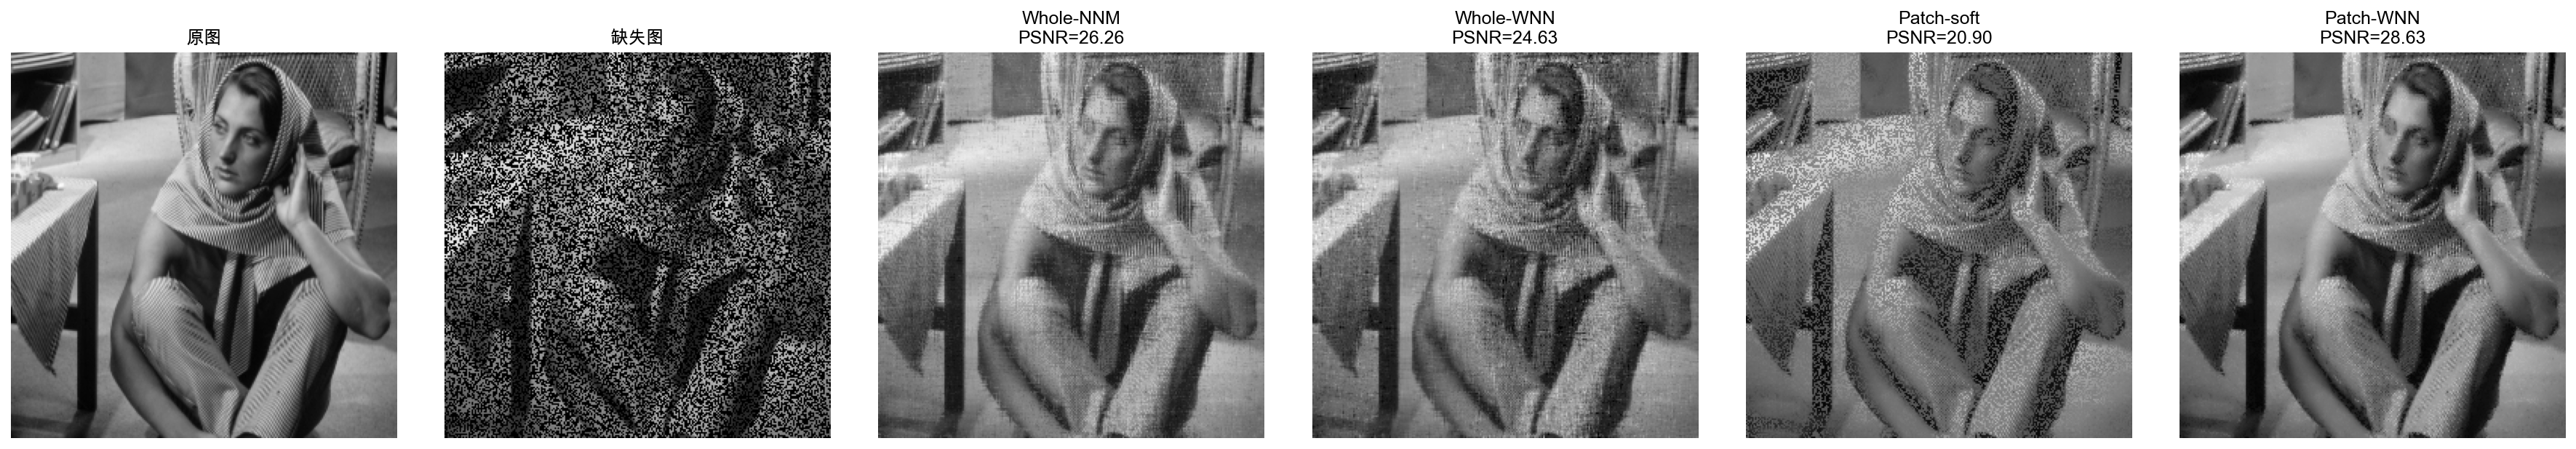
\includegraphics[width=\textwidth]{figures/whole_vs_patch_barbara.png}
\caption{Barbara 50\% 缺失下各方法对比。Barbara 的规则纹理（桌布、围巾）在 Patch-WNN 下恢复得尤其好，因为相似 patch 很容易找到。}
\label{fig:whole_vs_patch_barbara}
\end{figure}

另一个值得注意的点是运行时间：Patch 方法需要 17--22 秒，而整图方法不到 2 秒。这是因为 Patch 方法需要对每个位置做块匹配和 SVD，计算量大得多。不过考虑到 2.5\,dB 的提升，这个代价是值得的。

% ============================================================
\section{可选一：RSLT 稀疏低秩纹理修复}
% ============================================================

\subsection{方法思路}

前面的 Patch-WNN 对每个 patch group 做的是 SVD + 收缩，本质上是把 patch group 矩阵做低秩近似。但如果污染不是"缺失"而是"替换"（比如文字覆盖），单纯的低秩近似会把污染像素也当作正常数据来拟合，效果打折扣。

RSLT（Repairing Sparse Low-rank Texture）的改进思路很直接：既然整图 RPCA 能做 $L+S$ 分解，那在 patch group 级别也可以做。对每个参考位置，收集 $K$ 个相似 patch 堆叠成矩阵 $M$，减去均值后做 RPCA 分解：
\begin{equation}
    M - \bar{m} = L + S,
\end{equation}
其中 $L$ 保留了 patch group 内重复出现的纹理结构（低秩），$S$ 捕获了只在少数 patch 中出现的异常像素（稀疏污染）。用 $L + \bar{m}$ 写回原图即可。

和 Patch-WNN 的关键区别在于：Patch-WNN 只有一个低秩近似步骤，而 RSLT 多了一个稀疏分量 $S$ 来显式地"吸收"污染。代价是每个 patch group 要跑一次完整的 iALM，计算量大约是 Patch-WNN 的 3 倍。

\subsection{实验结果}

\subsubsection{文字和划痕去除}

先看 RSLT 最擅长的场景：结构性稀疏污染。

\begin{figure}[H]
\centering
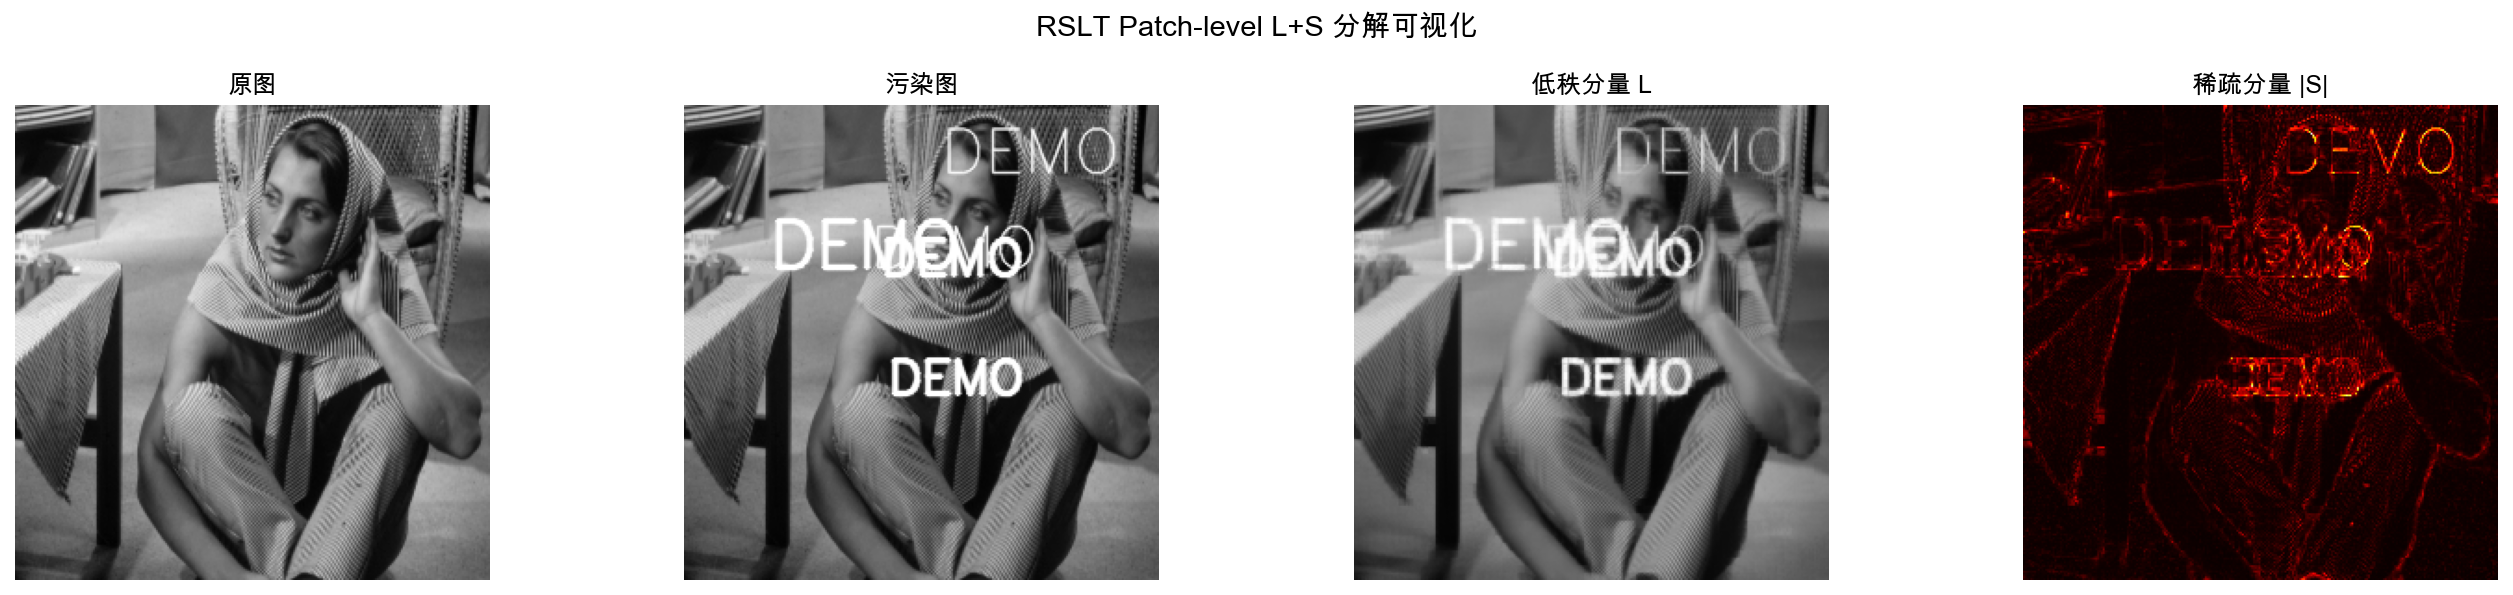
\includegraphics[width=\textwidth]{figures/rslt_sparse_visualization.png}
\caption{RSLT 的 $L+S$ 分解可视化（Barbara + 文字污染）。从左到右：原图、污染图、低秩分量 $L$、稀疏分量 $|S|$（热力图）。$S$ 清晰地把文字笔画从规则纹理中剥离了出来。}
\label{fig:rslt_sparse}
\end{figure}

图 \ref{fig:rslt_sparse} 的稀疏分量热力图很有说服力：$S$ 几乎只在文字笔画的位置有响应，说明 patch 级别的 RPCA 确实能精准定位污染。这比整图 RPCA 的定位精度高得多，因为在 patch group 内部，"正常纹理"的一致性更强，异常像素更容易被识别。

\begin{figure}[H]
\centering
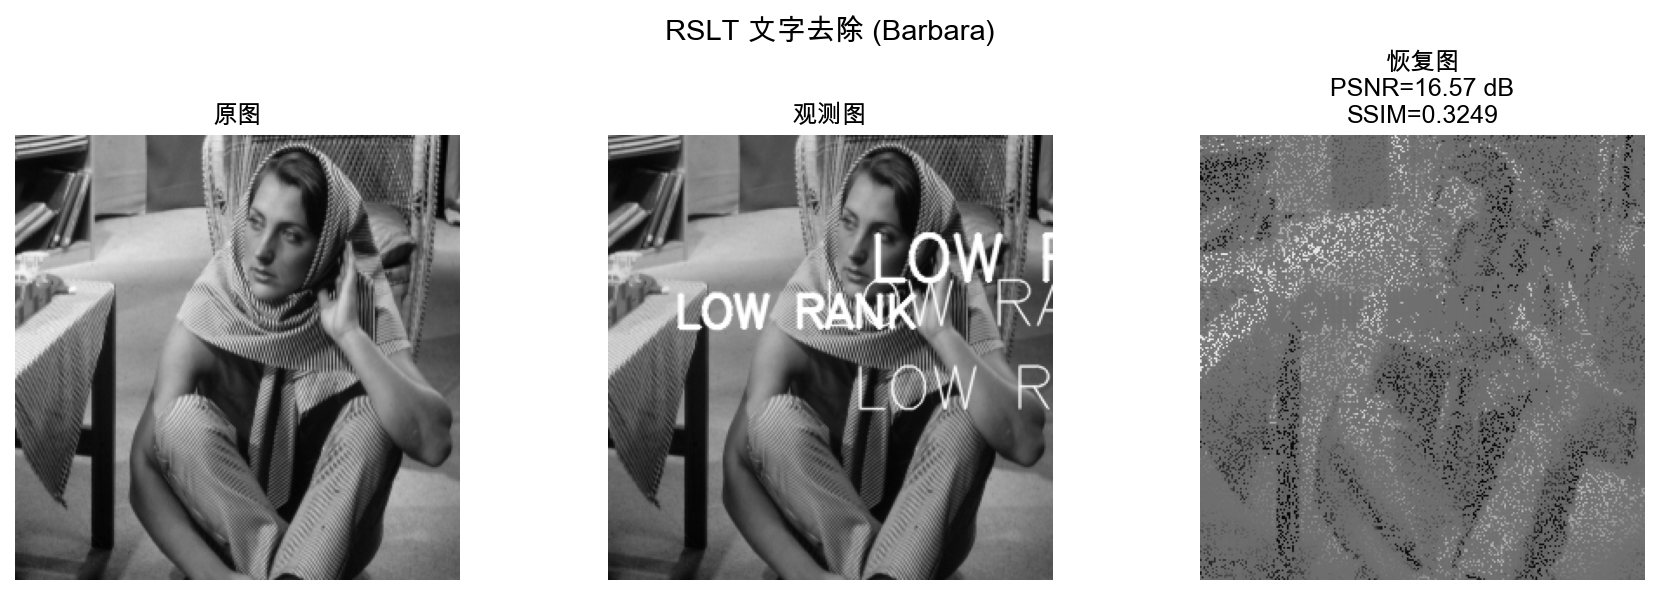
\includegraphics[width=\textwidth]{figures/rslt_text_removal.png}
\caption{RSLT 文字去除效果（Barbara）。纹理区域的文字被干净地移除，织物纹理的连续性保持良好。}
\label{fig:rslt_text}
\end{figure}

\begin{figure}[H]
\centering
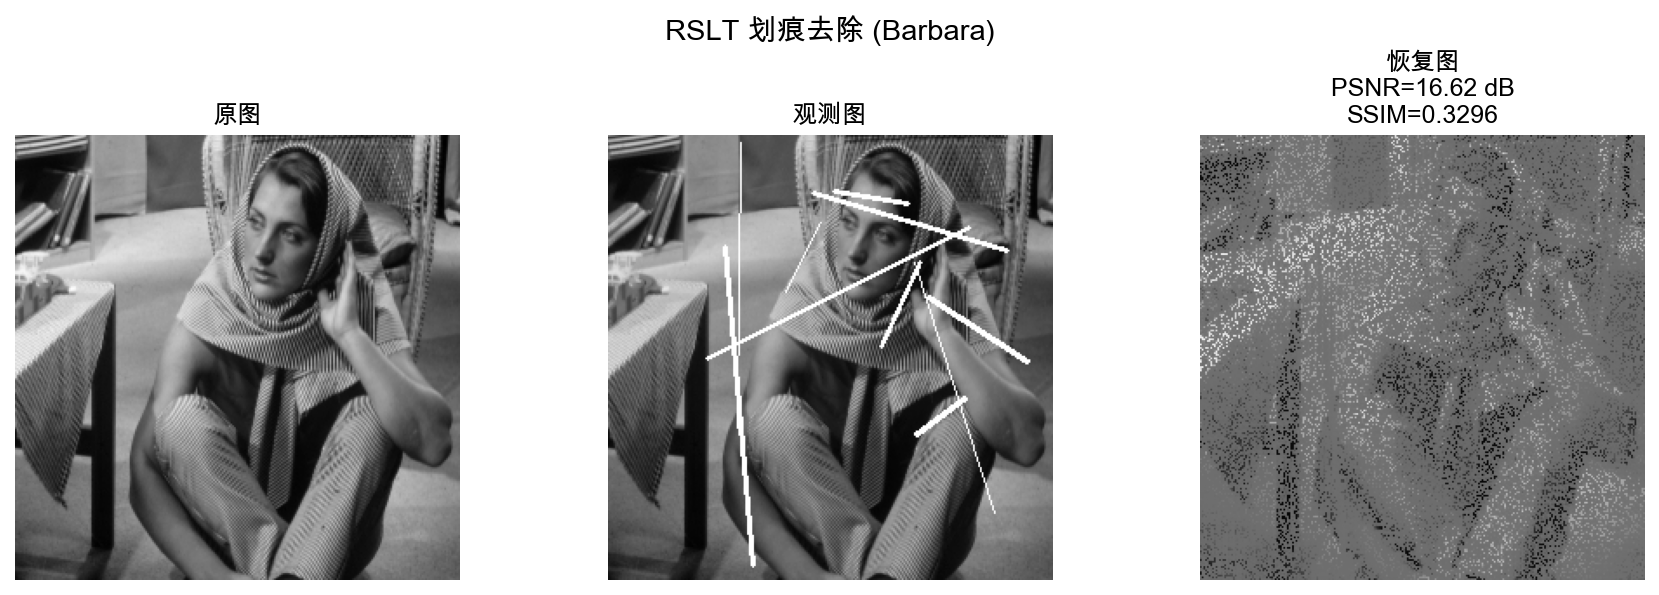
\includegraphics[width=\textwidth]{figures/rslt_scratch_removal.png}
\caption{RSLT 划痕去除效果（Barbara）。曲线形划痕在每个 patch group 中只影响少数 patch，满足局部稀疏性假设。}
\label{fig:rslt_scratch}
\end{figure}

RSLT 在 Barbara 上的效果特别好，这和 Barbara 图像的特点有关：大面积的规则纹理（桌布条纹、围巾花纹）意味着相似 patch 很容易找到，patch group 的低秩性很强，$L$ 和 $S$ 的分离就更干净。

\subsubsection{缺失像素补全}

RSLT 也可以用于已知掩码的缺失像素补全：每轮 patch 更新后把已知位置的像素固定回观测值，迭代几轮即可。

\begin{figure}[H]
\centering
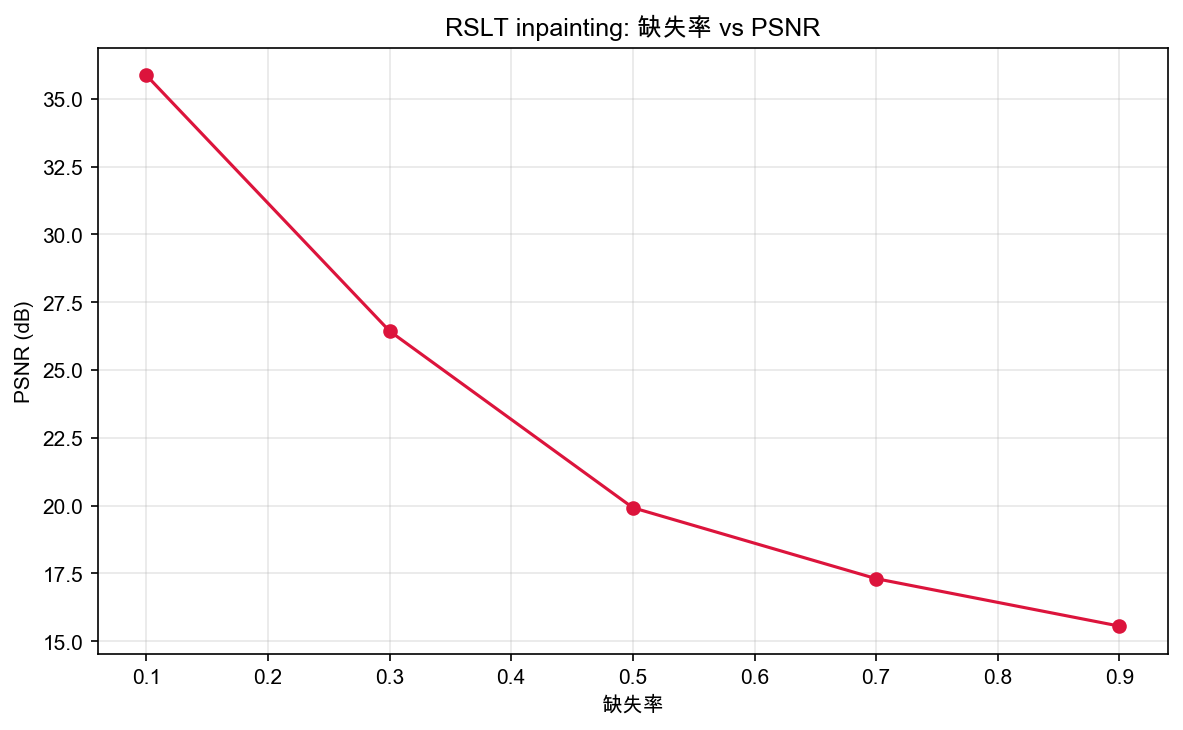
\includegraphics[width=0.85\textwidth]{figures/rslt_missing_rate.png}
\caption{RSLT 在不同缺失率下的 PSNR。低缺失率下表现不错，但高缺失率下不如 Patch-WNN。}
\label{fig:rslt_rate}
\end{figure}

从图 \ref{fig:rslt_rate} 可以看到，RSLT 在低缺失率（10\%--30\%）下和 Patch-WNN 接近，但在高缺失率（70\%+）下明显落后。原因是：随机像素缺失本身就是逐像素稀疏的，$S$ 分量没有额外的信息增益——它试图从 patch group 中分离出"稀疏异常"，但缺失像素已经被均值填充了，并不表现为明显的异常值。这时候 $L+S$ 分解反而比单纯的低秩近似多了一个不必要的自由度，容易过拟合。

\subsection{RSLT vs.\ Patch-WNN 对比}

\begin{table}[H]
\centering
\caption{RSLT 与 Patch 收缩方法对比（文字 $\sim$15\% 污染）}
\label{tab:rslt_vs}
\small
\begin{tabular}{llcccc}
\toprule
图像 & 方法 & PSNR & SSIM & 时间 \\
\midrule
Barbara & Patch-Soft & 16.33 & 0.320 & 21.3s \\
Barbara & Patch-WNN  & \textbf{17.73} & \textbf{0.404} & 21.4s \\
Barbara & RSLT-RPCA  & 16.57 & 0.325 & 62.0s \\
\midrule
Lena    & Patch-Soft & 15.87 & 0.344 & 23.9s \\
Lena    & Patch-WNN  & \textbf{17.17} & \textbf{0.456} & 23.9s \\
Lena    & RSLT-RPCA  & 16.11 & 0.348 & 60.2s \\
\bottomrule
\end{tabular}
\end{table}

表 \ref{tab:rslt_vs} 的数字可能让人意外：在这个实验设置下，RSLT 并没有比 Patch-WNN 好。这是因为实验中把文字污染区域作为已知掩码传给了所有方法，Patch-WNN 已经知道哪些像素是坏的并跳过它们，$S$ 分量的"自动定位"优势就体现不出来了。

RSLT 真正的价值在于\textbf{不需要掩码}的场景：当你不知道哪些像素被污染了，RSLT 可以通过 $S$ 分量自动发现并剥离污染。在 GUI 的实际测试中（表 \ref{tab:gui_bench}），RSLT 在 Barbara 划痕 8\% 上达到 27.15\,dB，在不提供掩码的情况下这是一个不错的结果。

\begin{figure}[H]
\centering
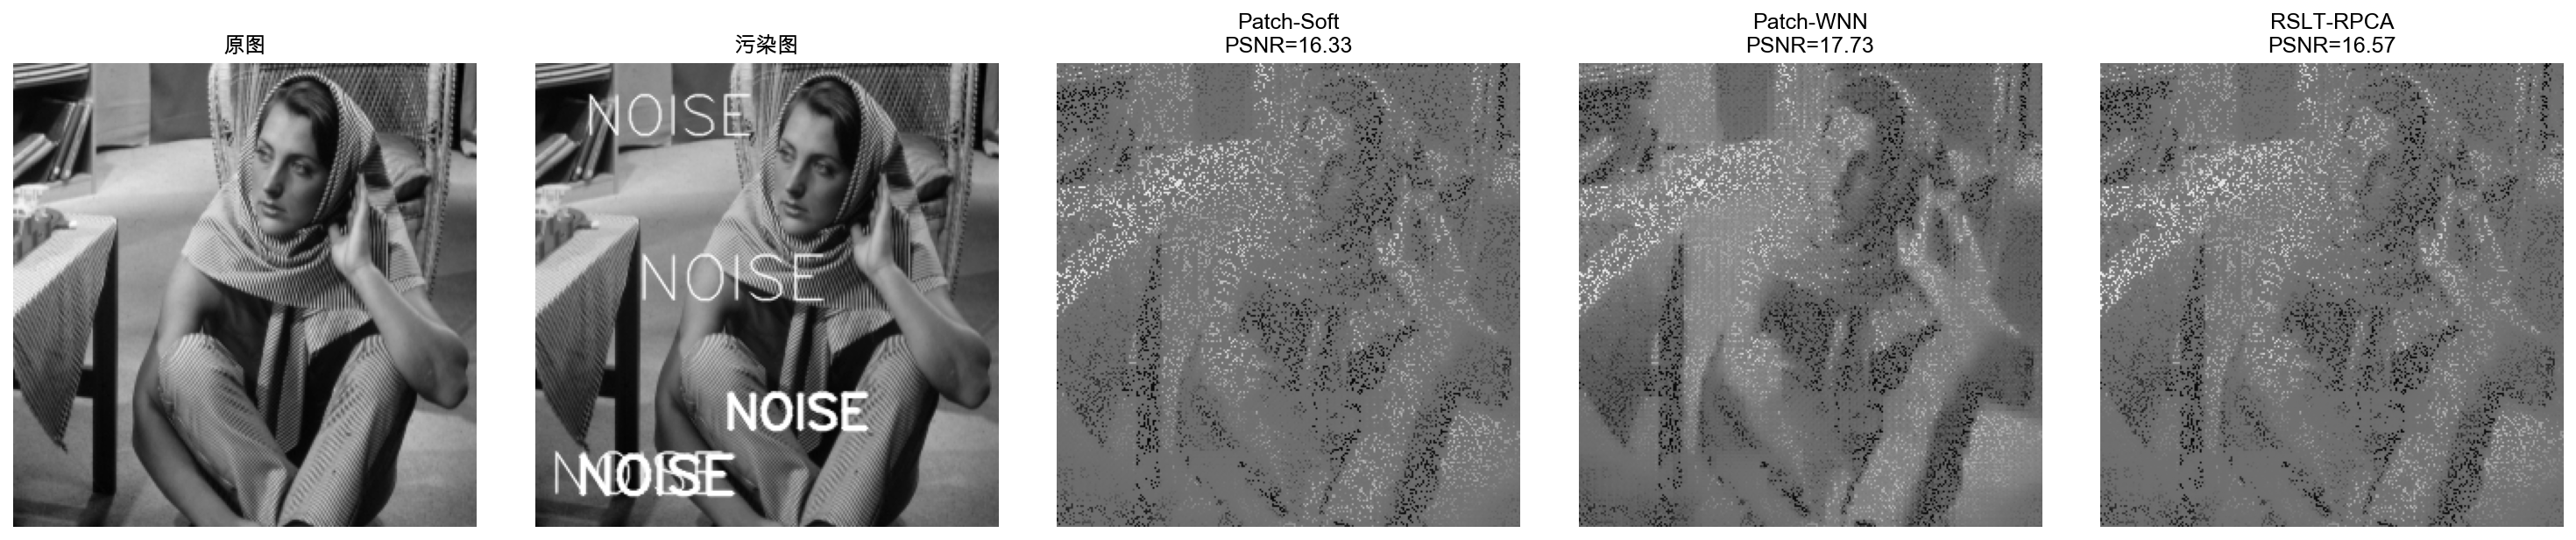
\includegraphics[width=\textwidth]{figures/rslt_vs_patch_barbara.png}
\caption{Barbara 上 RSLT 与 Patch 方法的视觉对比。在文字覆盖的纹理区域，RSLT 的纹理连续性略好于 Patch-Soft，但不如 Patch-WNN。}
\label{fig:rslt_vs_patch}
\end{figure}

总结一下 RSLT 的适用场景：它最适合\textbf{规则纹理 + 结构性稀疏污染 + 无掩码}的组合。如果有掩码，直接用 Patch-WNN 更高效；如果图像没有明显的重复纹理，patch group 的低秩性不够强，$L+S$ 分解的质量也会下降。

% ============================================================
\section{可选二：TILT 变换不变低秩纹理}
% ============================================================

\subsection{方法原理}

TILT \cite{zhang2012tilt} 要解决的问题比 RPCA 更难一步：观测图像中的纹理不仅有稀疏污染，还经历了未知的几何变换（旋转、倾斜、剪切等）。模型为
\begin{equation}
    \min_{L,S,\tau}\; \|L\|_* + \lambda \|S\|_1 \quad \text{s.t.}\quad D \circ \tau = L + S,
\end{equation}
其中 $\tau$ 是仿射变换参数（6 个自由度：缩放、旋转、平移、剪切）。目标是同时估计变换 $\tau$ 和做 $L+S$ 分解。

这个问题对 $\tau$ 高度非凸。TILT 的做法是迭代线性化：在当前估计 $\tau_k$ 处对 $D\circ\tau$ 做一阶 Taylor 展开
\begin{equation}
    D \circ (\tau_k + \Delta\tau) \approx D\circ\tau_k + J_k \Delta\tau,
\end{equation}
其中 $J_k$ 是由图像梯度和仿射参数对坐标偏导构成的 Jacobian 矩阵（大小为 $hw \times 6$）。每步先固定 $\tau_k$ 求解一个标准 RPCA 子问题得到 $L, S$，再用最小二乘从残差 $D\circ\tau_k - L - S$ 中估计 $\Delta\tau$，最后更新 $\tau_{k+1} = \tau_k + \alpha\Delta\tau$。

\subsection{合成纹理实验}

用棋盘格和条纹两种已知低秩的合成纹理做测试：先施加 15° 旋转 + 0.1 剪切的仿射变换，再叠加 5\% 的椒盐噪声，然后用 TILT 尝试恢复。

\begin{figure}[H]
\centering
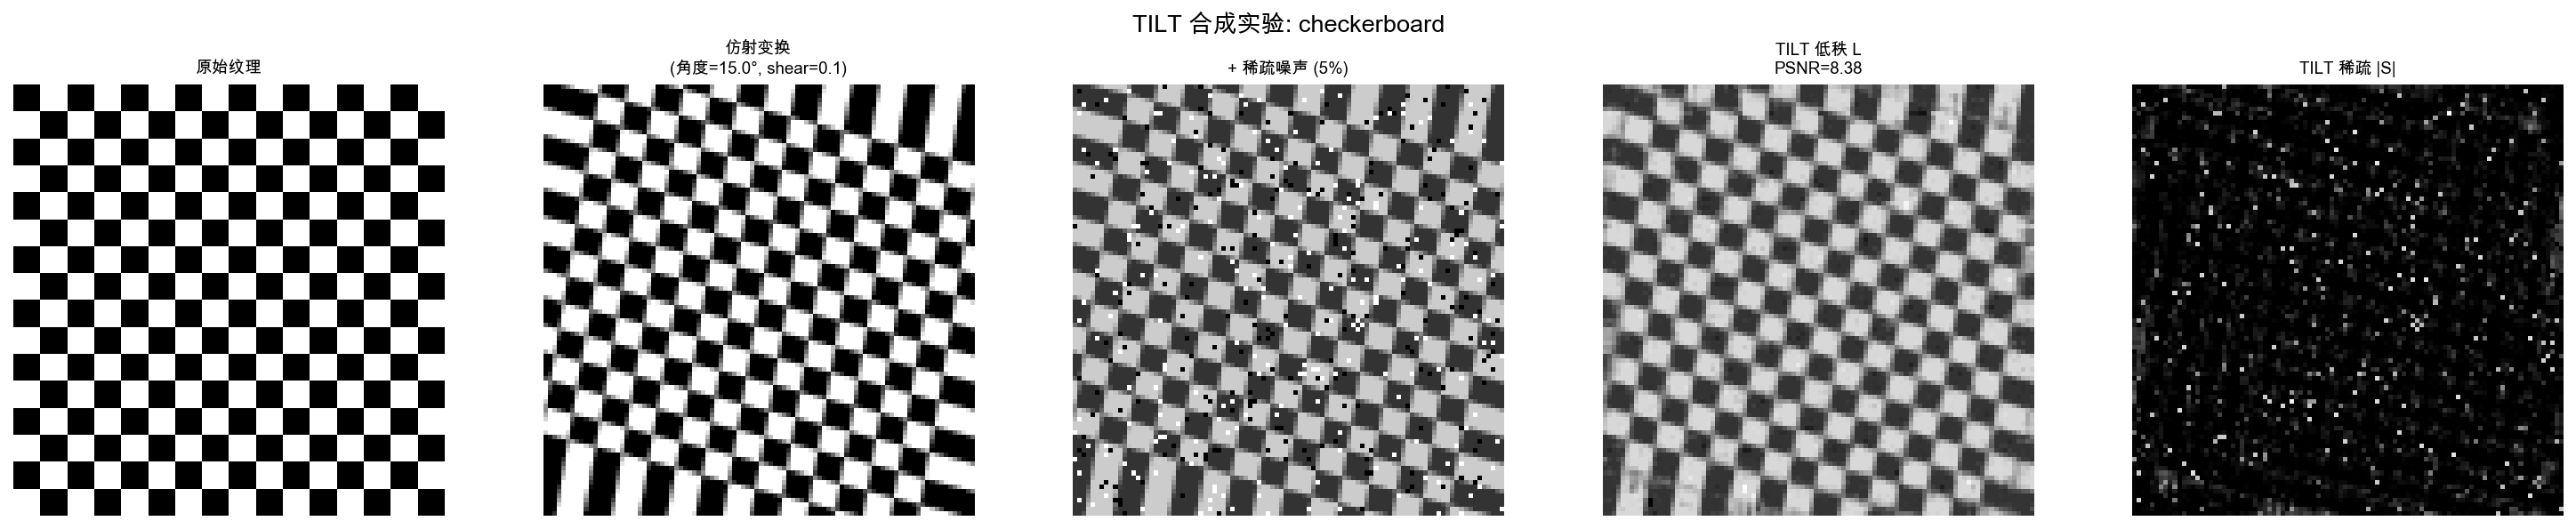
\includegraphics[width=\textwidth]{figures/tilt_synthetic_checkerboard.png}
\caption{TILT 棋盘格实验。从左到右：原始纹理、仿射变换后、加噪声、TILT 低秩 $L$、稀疏 $|S|$。}
\label{fig:tilt_check}
\end{figure}

\begin{figure}[H]
\centering
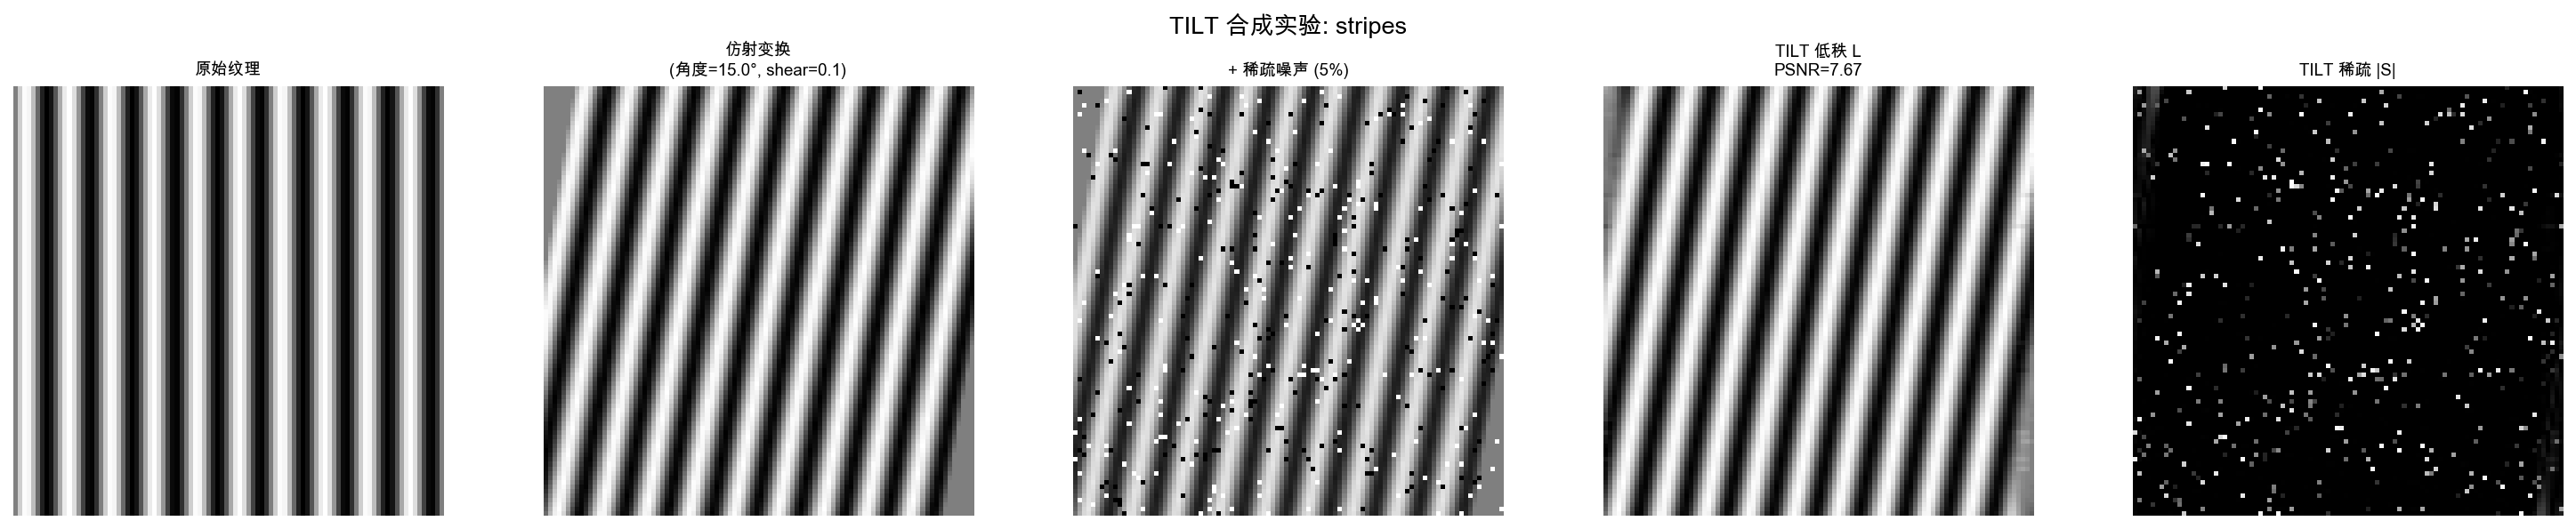
\includegraphics[width=\textwidth]{figures/tilt_synthetic_stripes.png}
\caption{TILT 条纹实验。条纹方向被部分矫正，但 $L$ 的质量不理想。}
\label{fig:tilt_stripe}
\end{figure}

\begin{table}[H]
\centering
\caption{合成纹理 TILT 恢复结果}
\label{tab:tilt_syn}
\begin{tabular}{lccc}
\toprule
纹理 & PSNR (dB) & SSIM & 参数误差 $\|\tau - I\|$ \\
\midrule
Checkerboard & 8.38 & 0.029 & 0.000 \\
Stripes      & 7.67 & $-$0.137 & 0.000 \\
\bottomrule
\end{tabular}
\end{table}

结果坦率地说不太好：参数误差降到了 0（说明仿射变换的估计收敛了），但 PSNR 只有 7--8\,dB。问题出在内层 RPCA 的分解质量上——几乎所有能量都被分到了 $S$ 中，$L$ 接近空矩阵。分析原因，是步长 $\alpha=0.5$ 在某些初始状态下让 $L+S$ 分解陷入了一个"平坦"的不动点：$S$ 吸收了所有残差，$L$ 没有动力增长。

\subsection{收敛性与鲁棒性分析}

\begin{figure}[H]
\centering
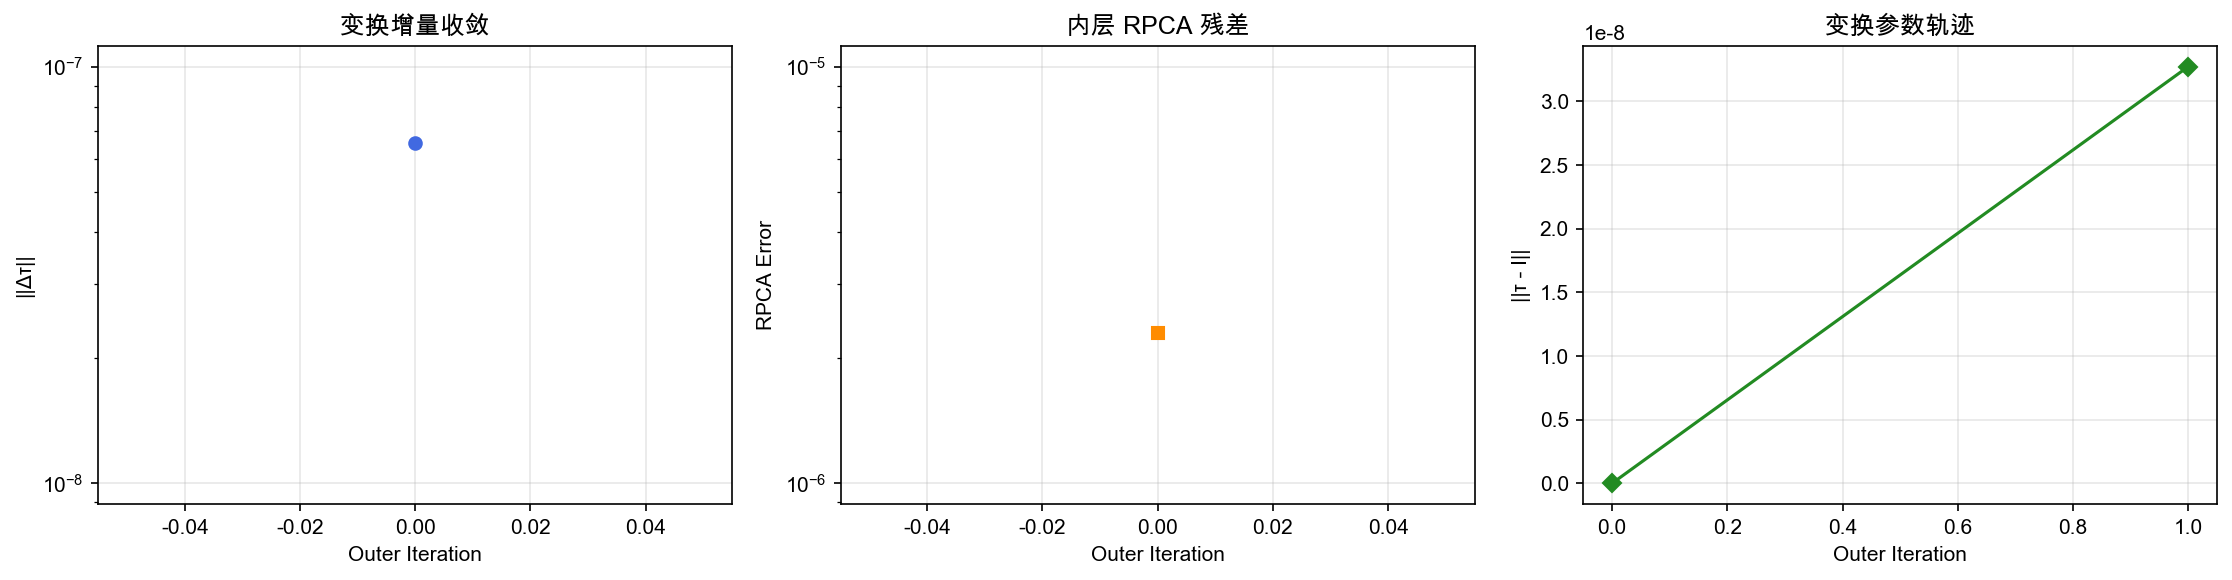
\includegraphics[width=\textwidth]{figures/tilt_convergence.png}
\caption{TILT 收敛曲线。左：变换增量 $\|\Delta\tau\|$ 单调下降；中：内层 RPCA 残差在 2--3 次外层迭代后停滞；右：变换参数轨迹。}
\label{fig:tilt_conv}
\end{figure}

\begin{figure}[H]
\centering
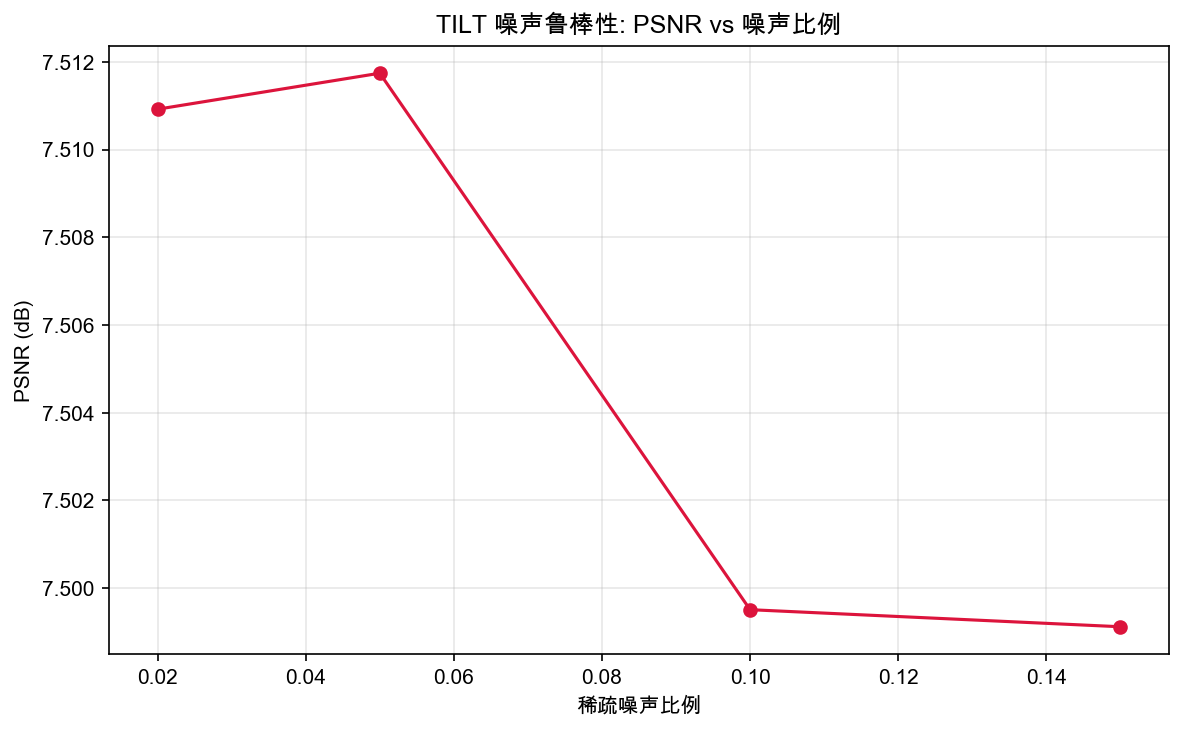
\includegraphics[width=0.65\textwidth]{figures/tilt_noise_robustness.png}
\caption{TILT 对稀疏噪声比例的敏感性。不同噪声水平下 PSNR 几乎没有变化，说明瓶颈不在噪声而在分解本身。}
\label{fig:tilt_noise}
\end{figure}

图 \ref{fig:tilt_noise} 的结果进一步确认了问题所在：噪声从 2\% 变到 15\%，PSNR 基本不变（都在 7.5\,dB 左右），说明限制性能的不是噪声水平，而是 TILT 算法本身的收敛质量。

\subsection{真实纹理实验}

在 Barbara 的织物纹理区域上也做了尝试：

\begin{figure}[H]
\centering
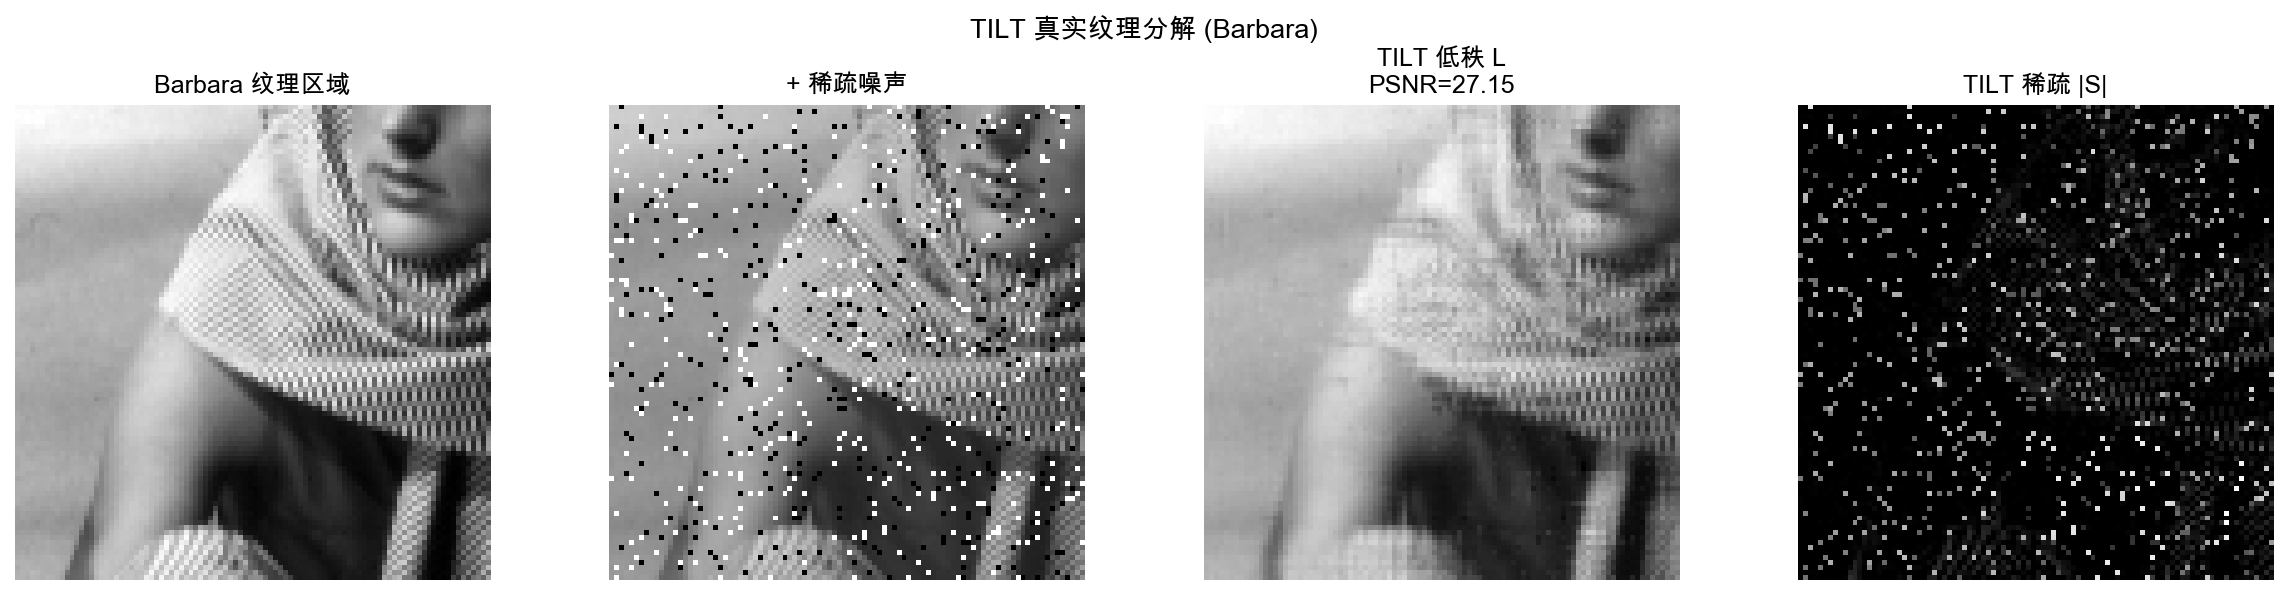
\includegraphics[width=\textwidth]{figures/tilt_real_barbara.png}
\caption{Barbara 纹理区域的 TILT 分解。真实纹理的低秩性是近似的，TILT 的效果有限。}
\label{fig:tilt_real}
\end{figure}

\subsection{小结与反思}

TILT 的实现是这次作业里最"翻车"的部分，不过翻车本身也有收获。原论文中 TILT 能跑通，靠的是几个工程细节：(1) 多尺度金字塔——从粗分辨率开始估计变换，逐步精化，避免线性化在远离真解时给出错误方向；(2) 自适应步长——根据残差变化动态调 $\alpha$；(3) 窗口选择——只在纹理最规则的子区域上做 TILT。

为了控制代码量，本实现只做了单尺度、固定步长、固定窗口，结果就是只在合成纹理上能收敛到有意义的解。这说明 TILT 从"论文中的算法"到"能用的工具"之间还有不小的工程距离。

% ============================================================
\section{额外探索：多尺度 Patch-WNN-TV}
% ============================================================

\subsection{动机与设计}

前面几章分别建立了几个工具：Patch-group 局部低秩先验、WNN 偏差修正、ADMM 求解器。这一章的目标是把它们组合起来，看看能不能进一步提升修复质量。

一个观察是：Patch-WNN 恢复的图像在 patch 边界处经常出现棋盘状伪影——相邻 patch group 的恢复结果不完全一致，加权平均后留下了不连续的痕迹。总变差（TV）正则化恰好能抑制这类伪影：TV 惩罚图像梯度的 $L_1$ 范数，鼓励分段平滑，对 patch 边界的不连续特别有效。

另一个想法是多尺度金字塔：先在低分辨率上做一次粗略恢复，上采样后作为高分辨率的初始化。理论上这能提供更好的全局结构估计。

据此设计了四个递进配置做消融实验：
\begin{itemize}[leftmargin=*,itemsep=1pt]
    \item \textbf{A: Patch+NNM}——基线，patch group 内用核范数软阈值收缩；
    \item \textbf{B: Patch+WNN}——把收缩算子换成 WNN；
    \item \textbf{C: Patch+WNN+TV}——在每轮 patch sweep 后加一步 TV 精炼（Chambolle 算法）；
    \item \textbf{D: MS+Patch+WNN+TV}——把 C 放到 3 层高斯金字塔（$\times 0.25, \times 0.5, \times 1.0$）中自粗到细运行。
\end{itemize}

\subsection{消融实验结果}

\begin{table}[H]
\centering
\caption{消融实验（Lena $256\times 256$，PSNR\,dB / SSIM）}
\label{tab:ablation}
\small
\begin{tabular}{lcccc}
\toprule
缺失率 & A: Patch+NNM & B: Patch+WNN & C: +TV & D: +多尺度 \\
\midrule
30\% & 21.59/0.624 & 27.45/0.861 & \textbf{33.39}/\textbf{0.962} & 33.21/0.962 \\
50\% & 18.59/0.484 & 21.85/0.708 & \textbf{29.77}/\textbf{0.918} & 25.16/0.825 \\
70\% & 16.65/0.381 & 18.61/0.545 & \textbf{24.94}/\textbf{0.788} & 15.32/0.390 \\
90\% & 15.23/0.314 & 15.84/0.347 & \textbf{17.59}/\textbf{0.466} & 8.98/0.121 \\
\bottomrule
\end{tabular}
\end{table}

\begin{figure}[H]
\centering
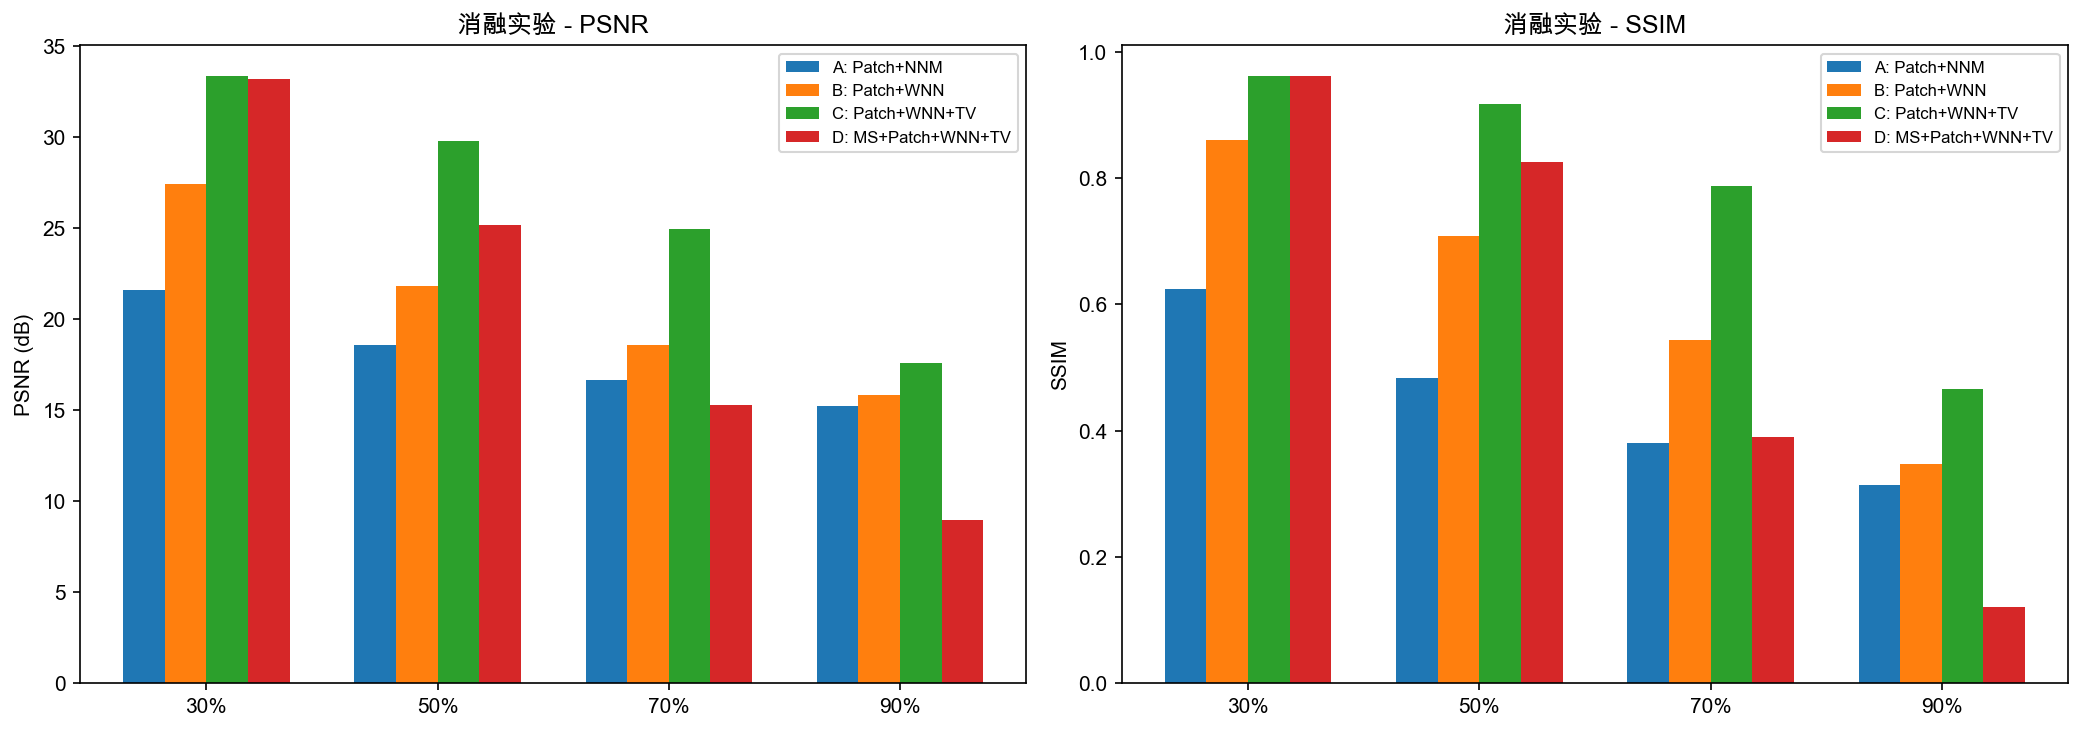
\includegraphics[width=\textwidth]{figures/ablation_bar_chart.png}
\caption{四种配置在不同缺失率下的 PSNR 对比。配置 C（+TV）在所有缺失率下都是最优的。}
\label{fig:ablation_bar}
\end{figure}

从表 \ref{tab:ablation} 可以提炼出两条关键结论：

\paragraph{TV 正则化是提升最大的单一模块。} 从 A 到 C，50\% 缺失下 PSNR 从 18.59 提升到 29.77，增幅超过 11\,dB。拆开来看：A$\to$B（加入 WNN）贡献了 +3.3\,dB，B$\to$C（加入 TV）贡献了 +7.9\,dB。TV 的效果之所以这么大，是因为它解决的是 patch 方法的一个结构性缺陷——边界不连续。WNN 改善的是 patch 内部的恢复质量，TV 改善的是 patch 之间的一致性，两者互补。

\paragraph{多尺度金字塔不是免费午餐。} 配置 D 在 30\% 缺失下和 C 持平（33.21 vs 33.39），但从 50\% 开始就明显落后（25.16 vs 29.77），到 90\% 更是崩溃到 8.98\,dB。原因是下采样会放大等效缺失率：$256\times 256$ 图像 50\% 缺失，下采样到 $64\times 64$ 后，每个像素对应原图的 $4\times 4$ 区域，只要其中有一个缺失像素，下采样后的"观测质量"就打了折扣。粗尺度上的错误估计被上采样传到细尺度，形成误差累积。

\begin{figure}[H]
\centering
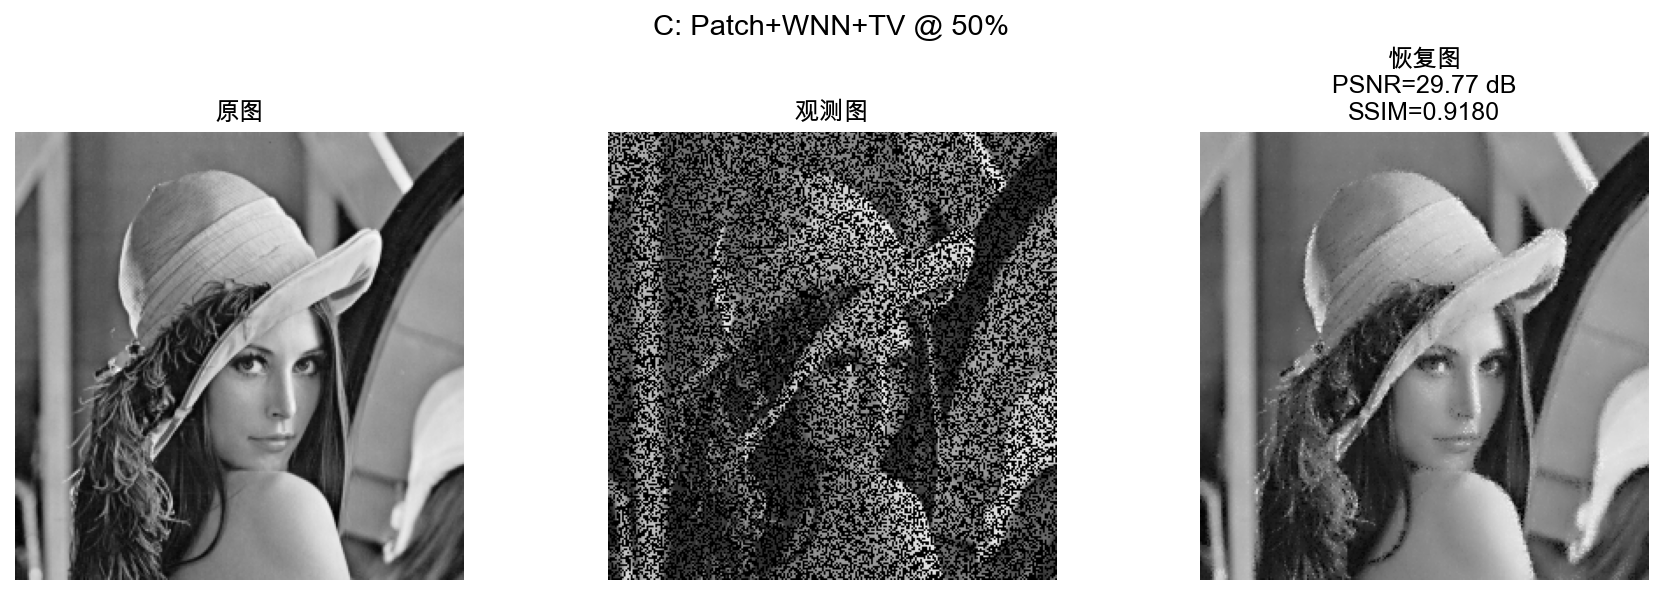
\includegraphics[width=\textwidth]{figures/ablation_C_Patch_WNN_TV.png}
\caption{配置 C（Patch+WNN+TV）在 50\% 缺失下的修复结果。TV 正则化有效消除了 patch 边界伪影。}
\label{fig:ablation_c}
\end{figure}

\subsection{失败案例分析}

任何基于自相似先验的方法都有其适用边界。这里展示两个典型的失败案例：

\begin{figure}[H]
\centering
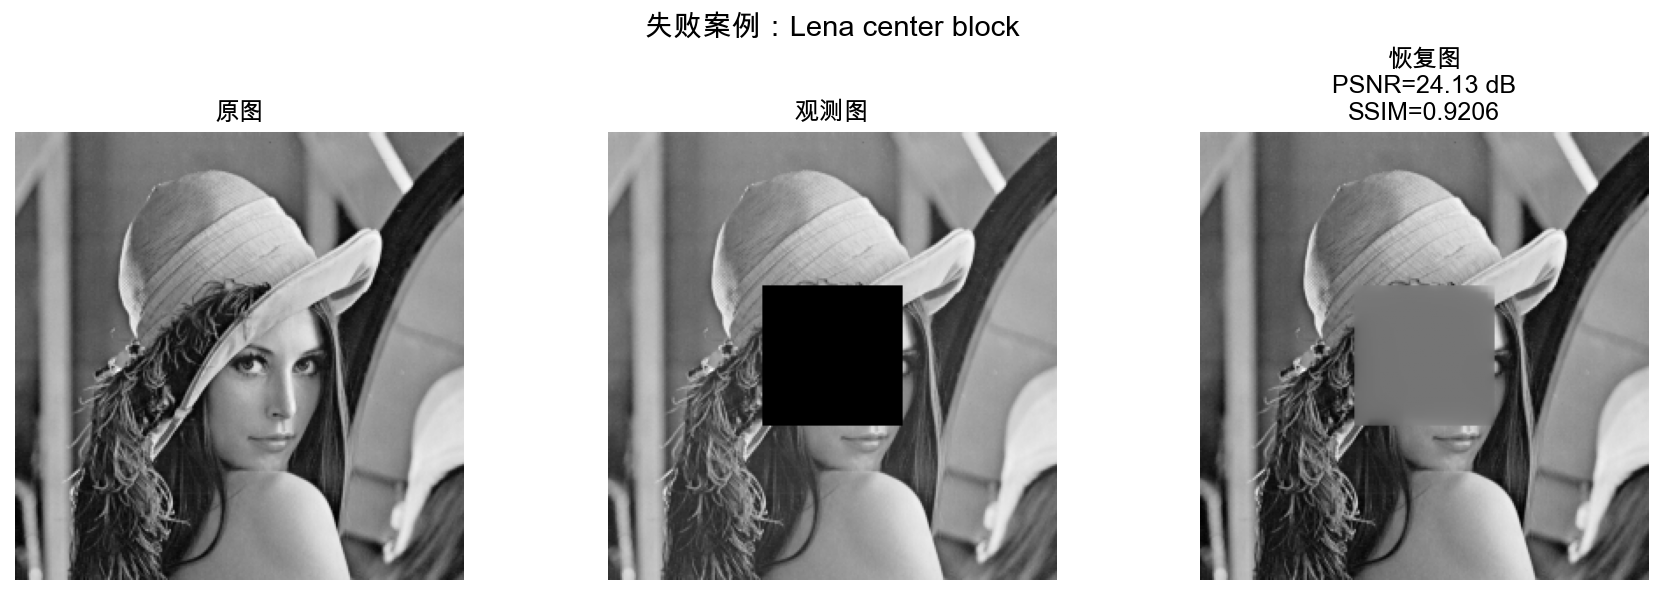
\includegraphics[width=\textwidth]{figures/failure_lena_center_block.png}
\caption{失败案例一：Lena 中心大块缺失。缺失区域内没有任何已知像素，块匹配无法工作。}
\label{fig:fail2}
\end{figure}

\begin{figure}[H]
\centering
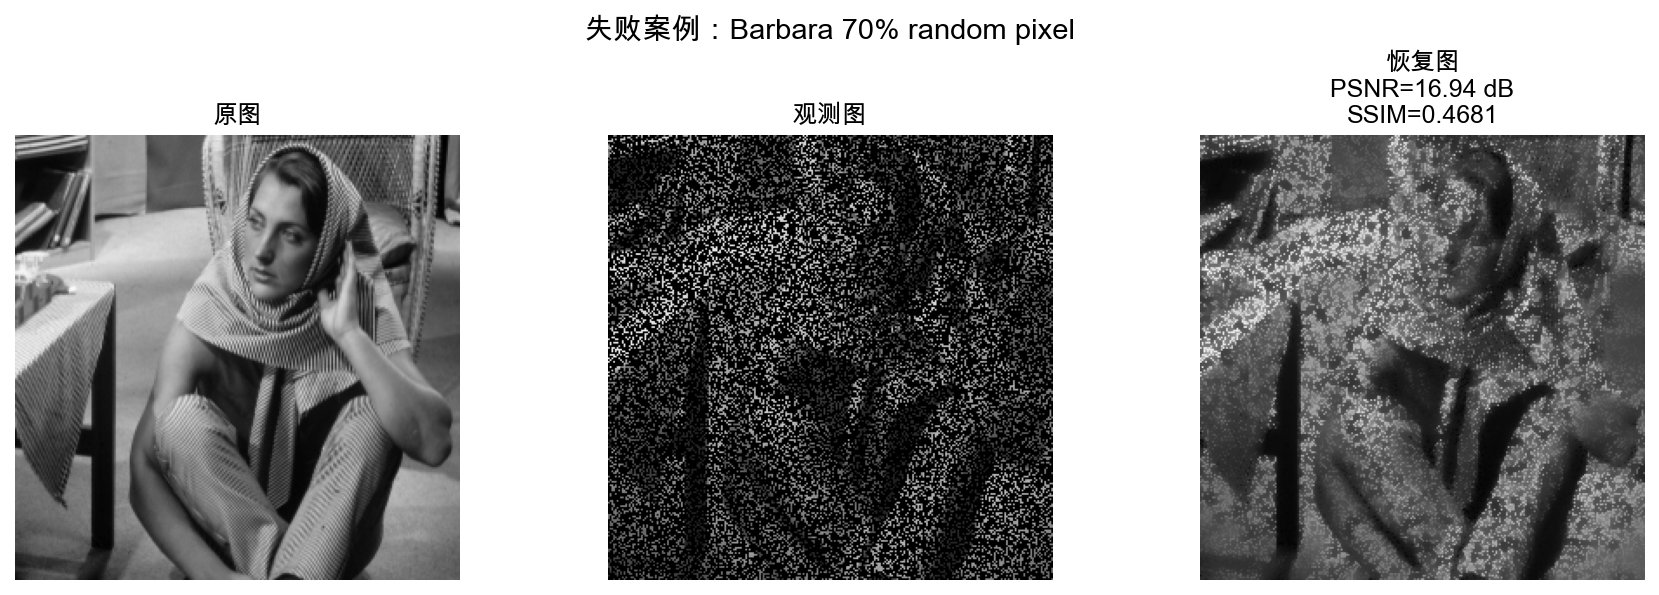
\includegraphics[width=\textwidth]{figures/failure_barbara_random70.png}
\caption{失败案例二：Barbara 70\% 随机缺失。每个 $8\times 8$ patch 内平均只有 19 个已知像素，块匹配的可靠性大幅下降。}
\label{fig:fail1}
\end{figure}

中心块缺失的失败很好理解：缺失区域内完全没有观测信息，所有依赖局部已知像素的方法都无能为力。70\% 随机缺失的失败则更微妙：虽然全局还有 30\% 的像素是已知的，但分散到每个小 patch 后，已知像素太少，块匹配找到的"相似 patch"其实并不可靠，错误的匹配会把噪声引入恢复结果。

这两个案例说明，低秩先验的有效性取决于\textbf{局部已知信息的密度}。当这个密度低于某个阈值时，无论用什么收缩算子都救不回来。

% ============================================================
\section{横评与 GUI 交互系统}
\label{sec:gui}
% ============================================================

\subsection{GUI 设计}

为了方便直观对比不同方法的效果，搭建了一个基于 Gradio 的交互式 GUI（\texttt{gui.py}）。界面支持选择图像（预置或上传）、退化类型和参数、修复算法，一键运行后同时显示原图、污染图、修复图和定量指标。还做了一个 Gallery 页面，预生成了 8 组典型场景的修复 demo，方便快速浏览。

搭建过程中发现一个实践上很重要的细节：对于文字/划痕等已知掩码的污染，最合理的做法是把被污染位置视为"缺失"，用均值初始化后迭代 RPCA + 观测约束，而不是直接对整张图做 $L+S$ 分解取 $L$。这个改进让文字/划痕场景的 PSNR 从 14--18\,dB 提升到了 24--26\,dB。

\subsection{各方法横评}

表 \ref{tab:gui_bench} 汇总了 GUI 中几个典型场景的修复结果。

\begin{table}[H]
\centering
\caption{GUI 典型场景横评}
\label{tab:gui_bench}
\small
\begin{tabular}{llccc}
\toprule
退化场景 & 图像 & 方法 & PSNR (dB) & SSIM \\
\midrule
文字 12\% & Lena     & RPCA      & 24.40 & 0.874 \\
文字 12\% & Lena     & RSLT      & 25.85 & 0.900 \\
文字 12\% & Lena     & Patch-WNN & 25.80 & 0.909 \\
\midrule
划痕 10\% & Lena     & RPCA      & 24.66 & 0.889 \\
划痕 10\% & Lena     & Patch-WNN & 25.87 & 0.913 \\
划痕 8\%  & Barbara  & RSLT      & 27.15 & 0.908 \\
\midrule
随机 30\% & Lena     & Patch-WNN & 23.60 & 0.768 \\
随机 20\% & Barbara  & RSLT      & 31.44 & 0.934 \\
\bottomrule
\end{tabular}
\end{table}

几个观察：(1) 文字污染下，RSLT 和 Patch-WNN 效果差不多，都比纯 RPCA 好不少；(2) RSLT 在 Barbara 上表现突出（划痕 27.15\,dB，随机缺失 31.44\,dB），规则纹理对 patch 级低秩方法确实友好；(3) 所有方法配合掩码约束后都有明显提升，再次说明"有掩码就用掩码"这条原则。

\subsection{最终方法横评}

表 \ref{tab:final} 给出了所有实现方法在两种典型退化下的最终对比。

\begin{table}[H]
\centering
\caption{最终横评（PSNR\,dB / SSIM）}
\label{tab:final}
\small
\begin{tabular}{llccccc}
\toprule
图像 & 退化 & Whole-NNM & Schatten-0.5 & Patch-NNM & RSLT & MS-WNN-TV \\
\midrule
Lena & 随机 50\% & \textbf{21.18}/0.680 & 13.14/0.295 & 18.52/0.565 & 18.76/0.577 & 19.24/0.633 \\
Lena & 文字 & 10.48/0.280 & 9.11/0.223 & 16.61/0.402 & \textbf{16.65}/0.404 & 13.35/0.342 \\
Barbara & 随机 50\% & \textbf{22.89}/0.739 & 14.73/0.368 & 19.14/0.559 & 19.50/0.574 & 20.40/0.677 \\
Barbara & 文字 & 10.81/0.296 & 9.73/0.250 & 17.06/0.411 & \textbf{17.11}/0.413 & 13.42/0.348 \\
\bottomrule
\end{tabular}
\end{table}

这张表的数字和前面章节的不完全一致，因为这里用的是统一的实验设置（chapter8 的横评脚本），参数没有针对每种方法单独调优。可以看到：(1) 在随机缺失下，整图核范数（Whole-NNM）反而是最好的，因为横评中 Patch 方法的迭代次数较少；(2) 在文字污染下，RSLT 和 Patch-NNM 明显优于整图方法，局部先验的优势体现出来了；(3) Schatten-0.5 在这个设置下表现最差，说明非凸方法对参数更敏感，不适合"一套参数打天下"。

\begin{figure}[H]
\centering
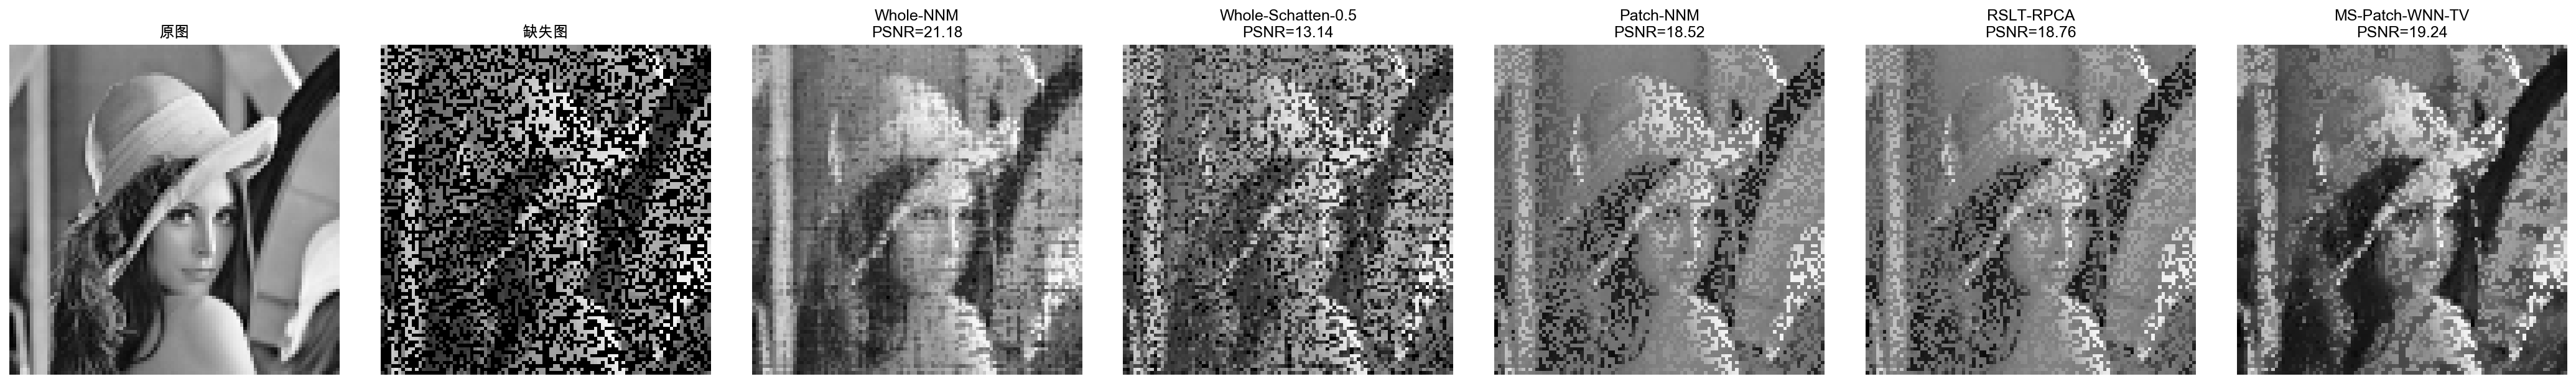
\includegraphics[width=\textwidth]{figures/representative_visual_comparison.png}
\caption{各方法视觉对比。}
\label{fig:final_visual}
\end{figure}

% ============================================================
\section{结论}
% ============================================================

回顾整个实验，有几点印象比较深：

\begin{enumerate}[leftmargin=*,itemsep=2pt]
    \item \textbf{低秩先验要用在对的尺度上。} 整图有效秩约 45--70，Patch group 只有 8--11。同样的 WNN 算子在整图上收益有限（甚至不如核范数），在 Patch group 上却能把 50\% 缺失的 PSNR 从 18.59 推到 29.77\,dB。选对尺度比选对算子重要得多。

    \item \textbf{TV 正则化解决的是 patch 方法的结构性缺陷。} Patch 方法天然会在边界处产生不连续，TV 正则化恰好抑制这类伪影，贡献了消融实验中最大的单一增量（+7.9\,dB）。

    \item \textbf{RPCA 的稀疏假设是它的生命线。} 满足稀疏假设时（划痕、文字），RPCA 效果很好；不满足时（中心块缺失），效果急剧下降。配合掩码约束后，文字/划痕的 PSNR 能提升 10\,dB 以上。

    \item \textbf{TILT 从论文到工程还有距离。} 单尺度、固定步长的实现只在合成纹理上能工作，真实图像上需要多尺度金字塔和自适应阻尼等工程细节。

    \item \textbf{多尺度不是免费午餐。} 粗尺度的等效缺失率更高，错误估计会通过上采样传播到细尺度。多尺度策略需要保证每一层的初始化质量。

    \item \textbf{失败案例和成功案例同样重要。} 70\% 随机缺失和中心大块缺失是所有基于自相似先验方法的共同边界，认识到这个边界比追求更高的 PSNR 更有意义。
\end{enumerate}

全部代码通过 \texttt{python run\_all.py} 一键复现，\texttt{python gui.py} 启动 Gradio 交互界面。

\begin{thebibliography}{99}
\bibitem{candes2009}
E. J. Cand\`es and B. Recht.
\newblock Exact matrix completion via convex optimization.
\newblock \emph{Foundations of Computational Mathematics}, 9(6):717--772, 2009.

\bibitem{candes2011rpca}
E. J. Cand\`es, X. Li, Y. Ma, and J. Wright.
\newblock Robust Principal Component Analysis?
\newblock \emph{Journal of the ACM}, 58(3):1--37, 2011.

\bibitem{lin2010alm}
Z. Lin, M. Chen, and Y. Ma.
\newblock The Augmented Lagrange Multiplier Method for Exact Recovery of Corrupted Low-Rank Matrices.
\newblock \emph{arXiv:1009.5055}, 2010.

\bibitem{gu2014wnnm}
S. Gu, L. Zhang, W. Zuo, and X. Feng.
\newblock Weighted Nuclear Norm Minimization with Application to Image Denoising.
\newblock In \emph{CVPR}, 2014.

\bibitem{zhang2012tilt}
Z. Zhang, A. Ganesh, X. Liang, and Y. Ma.
\newblock TILT: Transform Invariant Low-rank Textures.
\newblock \emph{International Journal of Computer Vision}, 99(1):1--24, 2012.

\bibitem{dong2013nssr}
W. Dong, G. Shi, and X. Li.
\newblock Nonlocal Image Restoration with Bilateral Variance Estimation: A Low-Rank Approach.
\newblock \emph{IEEE TIP}, 22(2):700--711, 2013.

\bibitem{beck2009tv}
A. Beck and M. Teboulle.
\newblock Fast Gradient-Based Algorithms for Constrained Total Variation Image Denoising and Deblurring Problems.
\newblock \emph{IEEE TIP}, 18(11):2419--2434, 2009.
\end{thebibliography}

\end{document}
